\documentclass[
    ngerman,
    color=3b,
    % dark_mode,
    % load_common, % Loads a list of commonly used Packages
    summary,
    boxarc,
    main,
]{rubos-tuda-template}
% Packages (nicht in Class File um CompileTime zu verbessern)
\usepackage[ngerman]{babel}
%\usepackage[utf8]{luainputenc} % if problems with ß exist
%\usepackage[table]{xcolor}  
\usepackage{makecell}
\usepackage{tikz-uml}
\usepackage{mleftright}
\usepackage{tikz}
\usepackage{placeins}
\usepackage{csquotes}
\usetikzlibrary{patterns, shapes, intersections, arrows, math, decorations,decorations.pathreplacing, decorations.pathmorphing, positioning, calc, automata, chains, matrix, arrows.meta, shapes.geometric, shadows.blur, shapes.symbols, backgrounds, tikzmark, angles}
\usepackage{nccmath}
\RequirePackage[framemethod=tikz]{mdframed} % Required for creating the theorem, definition, exercise and corollary boxes


% Definitionen für das Dokument (Bis auf studentEins alle Optional)
\title[SE]{Software Engineering}
\subtitle{Zusammenfassung}
\author{Ruben Deisenroth}
\contributor{Hendrik Rüthers} % List contributors here, seperate with \and
\semester{WiSe 2020/21}
\fachbereich{Informatik}
\version{1.0 (SNAPSHOT)}
\date{\today}
\termStyle{left-right-manual}
\termLeft{printAuthor,printContributor}
\termRight{printSemester,printVersion}
\term{\vspace{\baselineskip}\printDate{}\hfill\printFachbereich{}}
\ConfigureHeadline{
	headline={summary-centered}
}

% Workarounds and similar stuff.
\DeclareOldFontCommand{\it}{\normalfont\itshape}{\mathit}

\DeclareDocumentCommand{\resetrc}{}{\global\rownum=0\relax} % T#

% Dokument Anfang

\begin{document}

%--Titelseite--
\maketitle{}
\tableofcontents %Inhaltsverzeichnis

%% --Beginn Zusammenfassung--%%
\clearpage
\section{Einführung}
\subsection{Software}
\begin{definition}[Software]\index{Software}
    Der Begriff \textit{Software} bezeichnet ein Programm und all die dazugehörigen Daten, Informationen und Materialien. Das beinhaltet z.B.\begin{itemize}
        \item Ein (installierbares), ausführbares (operational) Programm und dessen Daten
        \item Konfigurationsdateien (configuration files)
        \item Systemdokumentationen (system documentation), z.B. Architekturmodell, Designvorstellungen, \dots
        \item Nutzerdokumentationen (user documentation), z.B. Anleitung, \dots
        \item Support (z.B. Wartung, Website, Telefon, \dots)
    \end{itemize}
    \hfill - W.S. Humphrey, SCM SIGSOFT, 1989
\end{definition}
\subsubsection{Arten von Software}
\begin{table}[ht]
    \centering
    \rowcolors{2}{\thepagecolor}{fgcolor!10!\thepagecolor}
    \newcommand{\tabitem}{~\llap{-}~}
    \begin{tabular}{rl}
        \toprule
        \fatsf{Typ}                          & \fatsf{Beschreibung}                                                            \\
        \midrule
        \fatsf{Application Software}         & \tabitem interagiert direkt mit dem Nutzer\continuerc                           \\
                                             & \tabitem Kann sowohl General purpose (z.B. Textverarbeitung, \dots)\continuerc  \\
                                             & ~~als auch anwendungsspezifisch (z.B. Kassensystem, \dots) sein                 \\
        \fatsf{System Level Software}        & \tabitem interagiert üblicherweise nicht direkt mit Nutzer\continuerc           \\
                                             & \tabitem Sorgt für funktionsfähiges System  (z.B. Treiber, \dots)               \\
        \fatsf{Software as a Service (SaaS)} & \tabitem Läuft auf einem Server\continuerc                                      \\
                                             & \tabitem Zugriff meist nur indirekt über Client (z.B. über Browser, SSH, \dots) \\

        \bottomrule
    \end{tabular}
    \caption{Arten von Software}\index{Softwaretypen}\index{Arten von Software}
    \label{tab:software:kinds}
\end{table}
\subsubsection{Softwarecharakteristiken}
\begin{itemize}
    \item Software nutzt sich nicht ab, aber muss sich ständig anpassen (z.B. an neue Hardware, \dots)
    \item Lebenszeit meist länger als erwartet (schwer zu bestimmen, da zukünftige Anforderungen ungewiss)
    \item Nur schwer messbar: Softwarequalität, Entwicklungsfortschritt und Zuverlässigkeit
\end{itemize}
\clearpage
\subsection{Engineering}
\begin{definition}[Engineering]\index{Engineering}
    (Entwickeln, Ingenieurswesen) bezeichnet den Prozess, wissenschaftliche Prinzipien zu nutzen, um Maschinen, Strukturen und viele weitere Dinge zu entwerfen.\\
    \phantom{a}\hfill - Cambridge Dictionary
\end{definition}
\begin{definition}[Software Engineering]\index{Software Engineering}
    ist ein Teilgebiet der Informatik und bezeichnet das Anwenden eines systematischen disziplinierten und qualifizierten Ansatzes der Entwicklung, Ausführung und Wartung der Software, sowie die Forschung und Entwicklung solcher Ansätze.
\end{definition}
\subsubsection{Characteristics of Engineering Approaches}
\begin{itemize}
    \item Fester/Definierter Prozess
    \item Getrennte Entwicklungsphasen, typischerweise: Analyse, Entwichlung (Design), Evaluation der Entwicklung, Konstruktion, Qualitätskontrolle (z.B. TÜV, oder mathematisch Korrektheit beweisen)
    \item Klare Trennung einzelner Teilsysteme
\end{itemize}
\subsubsection{Probleme der Softwareentwicklung}\index{Software Engineering!Probleme}
\begin{itemize}
    \item Kunde/Nutzer wenig/gar nicht an Entwicklung beteiligt
    \item Konstant verändernde Anforderungen an die Software
    \item Softwareentwickler oft nicht ausreichend geschult
    \item Managementprobleme
    \item Unpassende Methoden, Programmiersprachen, Tools
\end{itemize}
\clearpage
\section{Requirements Engineering}\index{Requirements engineering}
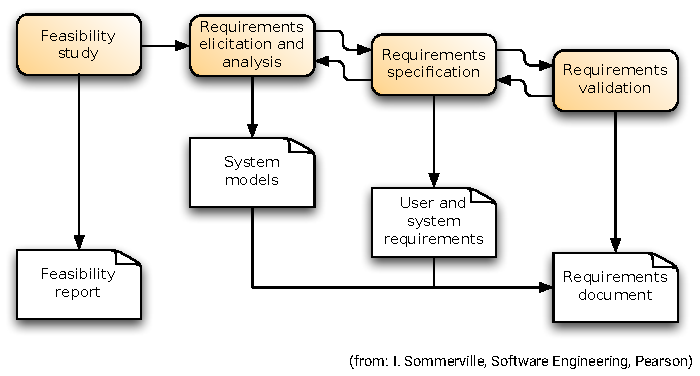
\includegraphics{bilder/Requirements engineering Process Flow.pdf}
{\centering
    \subsection{Anforderungsanalyse}\index{Requirements analysis}\index{Anforderungsanalyse}
}
\begin{definition}[Anforderungen]
    (requirements) sind die Beschreibungen der vom entworfenen System zu erfüllenden Aufgaben und dessen Einschränkungen
\end{definition}
Die Anforderungsanalyse beschäftigt sich mit dem Erkennen, der Analyse, der Dokumentation und der Validierung der Anforderungen.
\begin{itemize}
    \item Anforderungen werden in einem sog. Pflichtenheft (System Requirements Specification) festgehalten.
    \item use cases, state diagrams, usw werden im product backlog festgehalten.
    \item Anforderungen sind \textbf{keine} Lösungen/Implementierungen.
\end{itemize}
\subsubsection{Nutzeranforderungen (User requirements)}\index{User requirements}
\begin{itemize}
    \item beschreiben Aufgaben und Einschränkungen in Natürlicher Sprache oder mit Diagrammen (meist von Kunden geschrieben)
\end{itemize}
\fatsf{Beispiel:} Das System soll alle Buchungen speichern, so wie es das Gesetz verlangt.
\subsubsection{Systemanforderungen (System Requirements)}\index{Systemanforderungen}\label{System Requirements}
\begin{itemize}
    \item Präzise und detaillierte Beschreibung von  Aufgaben und Einschränkungen des Programmes (meist von Entwicklern geschrieben)
    \item Verfeinerung der Nutzeranforderungen
\end{itemize}
\fatsf{Beispiel:} Die Buchungen müssen für 10 Jahre gespeichert werden ab dem Zeitpunkt der Buchung.
\subsubsection{Domänenanforderungen (Domain Requirements)}\index{Domänenanforderungen}\label{Domain Requirements}
\begin{itemize}
    \item Meist nicht vom Kunden oder Entwickler spezifiziert, sondern von der Domäne (z.B. vom Gesetzgeber, \dots)
\end{itemize}
\fatsf{Beispiel:} Für die polizeiliche Ermittlung muss in Deutschland jede Transaktion für 2 Wochen zwischengespeichert werden.
\subsubsection{Funktionale Anforderungen (Functional Requirements)}\index{Funktionale Anforderungen}\label{Functional Requirements}
\begin{itemize}
    \item Die Dienste, die das System machen können soll
    \item die Reaktion des Systems auf bestimmte Eingaben und
    \item das Verhalten des Systems in bestimmten Situationen.
\end{itemize}
\fatsf{Beispiel:} Wenn der Nutzer den Knopf "`Neues Dokument"' drückt, wird eine neues Textdokument angelegt.
\subsubsection{Nichtfunktionale Anforderungen (Non-Functional Requirements)}\index{Nichtfunktionale Anforderungen}\label{Non-Functional Requirements}
Spezifizieren Einschränkungen der Dienste/Funktionen des Systems, welche oft nicht vollständig von Tests abgedeckt werden können:
\begin{itemize}
    \item Produktanforderungen (Product requirements)\index{Product requirements}\begin{itemize}
              \item Portabilität (Läuft auf verschiedenen Plattformen/lässt sich leicht darauf anpassen)
              \item Zuverlässigkeit/Robustheit (Reagiert auch auf unvorhergesehene/Illegale Eingaben und Situationen sinvoll)
              \item Effizienz (Leistung, Speicherplatz)
              \item Nutzbarkeit (Verständlichkeit, \dots)
          \end{itemize}
    \item Organisatorische Anforderungen(Organisational requirements)\begin{itemize}\index{Organisational requirements}
              \item Auslieferungsanforderungen
              \item Implementation
              \item Nutzung von Standards (ISO, IEEE, \dots)
          \end{itemize}
    \item Externe Anforderungen (External requirements)\index{External requirements}\begin{itemize}
              \item Interoperabilität (Interoperability requirements), d.h. Zusammenspiel mit anderen Systemen
              \item Ethische Anforderungen
              \item Rechtliche Anforderungen (Datenschutz, Sicherheit, \dots)
          \end{itemize}
\end{itemize}
Nichtfunktionale Anforderungen sind oftmals großflächige Anforderungen, welche das gesamte System betreffen. Allerdings sind solche Anforderungen meistens kritischer als funktionale Anforderungen
(bspw. "`Das System soll sicher vor Angriffen sein."').\\
Um nichtfunktionale Anforderungen überprüfbar zu machen, ist oftmals eine Umformulierung oder
Abänderung der eigentlichen Anforderung nötig. Hierdurch können auch funktionale Anforderungen
aufgedeckt werden.\\
\fatsf{Beispiel:} Die Oberfläche soll ansprechend und einfach zu bedienen sein.
\clearpage
\subsubsection{RE-Prozess}
\fatsf{Viewpoint-Oriented approach}
\begin{itemize}
    \item Interactor viewpoints: direktes Interesse
    \item Indirect viewpoints: indirektes Interesse
    \item Domain viewpoints: indirektes Interesse
\end{itemize}
\begin{definition}[FURPS+ Modell]\index{FURPS+ Modell}
    Functionality, Usability, Reliability, Performance, Supportability\\Plus Implementation (Interface,Operations,Packaging,Legal)
\end{definition}
\fatsf{Anforderungsvalidierung (Requirements validation checks)}\begin{itemize}
    \item Korrektheit (Validity): Beinhalten die Anforderungen alle nötigen Funktionen oder werden weitere benötigt?
    \item Konsistenz: Gibt es Konflikte bei den Anforderungen?
    \item Komplettheit: Sind alle Funktionen und Einschränkungen wie erwünscht angegeben?
    \item Realisierbarkeit (Realism): Sind die Anforderungen realistisch erfüllbar?
    \item Testbarkeit (Verifiability): Lässt sich das Erfüllen der Anforderungen testen?
    \item Verfolgbarkeit (Tracability): Lässt sich nachvollziehen, warum die Anforderung existiert?
\end{itemize}
\section{Anwendungsfälle (Use Cases)}
\subsection{Use Case Analysis}
\begin{definition}[Anwendungsfälle] (Use Cases)
    beschreiben, wie ein Angehöriger einer Rolle (\textit{Akteur}) das System in einem bestimmten \textit{Szenario} nutzt.
\end{definition}
\subsubsection{Requirements vs Use Cases}
\begin{table}[ht]
    \centering
    \rowcolors{2}{\thepagecolor}{fgcolor!10!\thepagecolor}
    \resetrc{}
    \begin{tabular}{ll}
        \toprule
        \fatsf{Requirements}                                      & \fatsf{Use Cases}                                                 \\
        \midrule
        ~\llap{-}~Fokus auf gewünschte \textit{Funktionalität}    & ~\llap{-}~Fokus auf mögliche \textit{Szenarios}                   \\
        ~\llap{-}~Werden meist einfach deklariert (declaratively) & ~\llap{-}~Werden anhand von Szenarios beschrieben (operationally) \\
        ~\llap{-}~Perspective des Clients                         & ~\llap{-}~ Perspektive des Users                                  \\
        \bottomrule
    \end{tabular}
    \caption{Requirements vs Use Cases}
    \label{tab:requirements_vs_use_cases}
\end{table}
\begin{itemize}
    \item Ohne Nutzerbeteiligung nahezu unmöglich, gute/vollständige Anwendungsfälle zu schreiben
    \item Anwendungsfälle ergänzen die Anforderungsanalyse, ersetzen sie aber nicht (können keine nichtfunktionalen Anforderungen erfassen)
\end{itemize}
\subsubsection{Use Case Formats}
\begin{itemize}
    \item kurz (brief): Kurze Zusammenfassung, normalerweise das Haupterfolgsszenario
    \item informell (casual): Informelles Format, mehrere Zeilen die mehrere Szenarios behandeln
    \item ausgearbeitet (Fully dressed): Alle Zwischenschritte und Variationen sind im Detail aufgeschrieben, es gibt hilfssektionen, z.B. Vorbedingungen (preconditions) und Erfolgsgarantien (sucess guarantees)
\end{itemize}
Ein vollständig ausgearbeiteter Anwendungsfall sieht so aus:
\begin{table}[ht]
    \centering
    \rowcolors{2}{\thepagecolor}{fgcolor!10!\thepagecolor}
    \resetrc{}
    \begin{tabular}{ll}
        \toprule
        \fatsf{Abschnitt}                            & \fatsf{Beschreibung/Einschränkung}                        \\
        \midrule
        Use Case Name                                & Der Name des Anwendungsfalls / Startet mit einem Verb     \\
        Bereich (Scope)                              & Betroffener Bereich des Systems                           \\
        Ebene (Level)                                & Abstraktionsebene/ \continuerc                            \\
                                                     & Nutzerziel, Zusammenfassung oder Unterfunktion            \\
        Hauptakteur (Primary actor)                  & Initiator des Anwendungsfalls                             \\
        Stakeholders and Interests                   & Personen, die dieser Anwendungsfall betrifft              \\
        Vorbedingungen (preconditions)               & Was muss beim start des Programmes gelten?\continuerc     \\
                                                     & Ist es das Wert dem Leser mitzuteilen?                    \\
        Akzeptanzkriterien (Minimal Guarantee)       & Minimalversprechen an Stakeholders                        \\
        Erfolgskriterien (Success Guarantee)         & Was sollte das Programm können, wenn es erfolgreich ist?  \\
        Haupterfolgsszenario (Main Success Scenario) & Typischer Ablauf des Szenarios /\continuerc               \\
                                                     & Nummerierte Schrittliste um das Ziel zu erreichen         \\
        Erweiterungen                                & Alternative Erfolgs- und Fehlschlagszenarien /\continuerc \\
                                                     & Fehlschlagspunkte des Hauptszenarios                      \\
        \tikzmark{A}Spezialanforderungen             & Verwandte, nichtfunktionale Anforderungen                 \\
        Technologien                                 & Einzusetzende Technologien                                \\
        Häufigkeit (Frequency of occurrence)         & Häufigkeit des Eintretens des Anwendungsfalls             \\
        \tikzmark{B}Anderes (Misc)                   & Bspw. offene Tickets                                      \\
        \bottomrule
    \end{tabular}
    \begin{tikzpicture}[remember picture, overlay]
        \draw[thick,decorate,decoration={brace,amplitude=8pt,raise=6pt, mirror}, accentcolor]([yshift=.9em]pic cs:A)-- ([yshift=-.3em]pic cs:B)node[midway, xshift = -1.1cm,align=left]{nicht\\immer\\nötig};
    \end{tikzpicture}
    \caption{Fully Dressed Use Case schema}
    \label{tab:fully_dressed_use_case}
\end{table}
\subsubsection{Richtlinien für das Entwickeln von Anwendungsfällen}
\begin{enumerate}
    \item Akteure und deren Interessen aufzählen $\Longrightarrow$ Erste Ebene an Präzission
    \item Stakeholders, Trigger (Erster Schritt des Haupterfolgsszenarios), Validieren $\Longrightarrow$ Zweite Ebene an Präzission
    \item Alle Fehlschlagszenarien identifizieren und auflisten
    \item Fehlerbehandlung schreiben
\end{enumerate}
\clearpage
\subsection{UML Nutzungszweck Diagramme (UML Use Case Diagrams)}
\begin{definition}[Unified Modeling Language (UML)]\index{UML}
    Visuelle, aber präzise Entwurfsschreibweise für Softwareentwicklung
    \begin{itemize}
        \item Hauptziel: Objektmodellierung vereinheitlichen, indem sich auf eine feste Syntax und Semantik geeinigt wird
    \end{itemize}
\end{definition}
\begin{definition}[Nutzungszweck-Diagramm (Use case Diagram)]
    Stellt Anforderungsfälle und deren Relationen zu dem System und dessen Akteuren dar.
\end{definition}
\begin{table}[ht]
    \centering
    \rowcolors{2}{\thepagecolor}{fgcolor!10!\thepagecolor}
    \resetrc{}
    \begin{tabular}{cl}
        \toprule
        \fatsf{Element}                                                              & \fatsf{Beschreibung}                                                                \\
        \midrule
        \raisebox{-.5\height}{
\includegraphics[height=3cm]{bilder/uml/actor.pdf}}    & Stellt einen Akteur innerhalb des Systemes dar.                                     \\
        \raisebox{-.5\height}{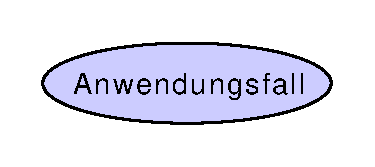
\includegraphics[height=2cm]{bilder/uml/use_case.pdf}} & Stellt einen Anwendungsfall im System dar                                           \\
        \raisebox{-.5\height}{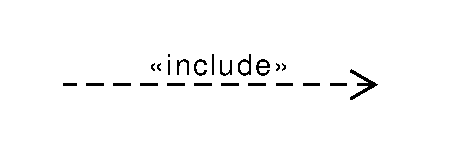
\includegraphics[height=2cm]{bilder/uml/include.pdf}}  & \Gape[0pt][2pt]{\makecell[l]{Erweitert einen Anwendungsfall um eine Funktionalität. \\
        Wird der erweiterte Anwendungsfall "`ausgeführt"',                                                                                                                 \\
        so wird auch dieser Anwendungsfall "`ausgeführt"'.}}                                                                                                               \\
        \raisebox{-.5\height}{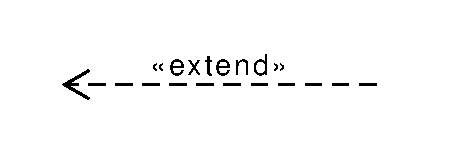
\includegraphics[height=2cm]{bilder/uml/extend.pdf}}   & \Gape[0pt][2pt]{\makecell[l]{Erweitert einen Anwendungsfall um eine Funktionalität. \\Ist die Bedingung in der Beschreibung wahr, so wird der \\ erweiternde Anwendungsfall mit "`ausgeführt"'.}}\\
        \bottomrule
    \end{tabular}
    \caption{Use Case Diagram Elemente}
    \label{tab:use_case_diagram_elements}
\end{table}
\paragraph{Beispiel}\mbox{}\\
In einem Autohandel ist es möglich, sowohl Bar als auch mit Kreditkarte zu zahlen. Auch ist es dem Kunden möglich, Automobile zu mieten. Da der Handel neue Kunden gewinnen möchte, ist es ab sofort möglich, bei dem Mieten eines Autos Treuepunkte zu sammeln. Dem Ladeninhaber ist es möglich, neue Autos in das Sortiment aufzunehmen. Wurde ein Ausstellungsauto einmal gemietet, so sinkt der Kaufpreis von diesem. \\ \textit{Diese Anforderungen sind in \figurename{} \ref{fig:usecase} dargestellt.}
\begin{figure}[ht]
    \centering
    \begin{tikzpicture}
        \umlactor[x = -8, y = 0]{Kunde}
        \umlactor[x = 8, y = -6]{Inhaber}
        \begin{umlsystem}[x = 0, y = 0]{Autohandel}
            \umlusecase[x = 0, y = 2, name = buy]{Auto kaufen}
            \umlusecase[x = 0, y = -2, name = rent, width = 2.7cm]{Auto mieten \\ EP: Treuepunkte}
            \umlusecase[x = 0, y = -7, name = add]{Auto aufnehmen}
            \umlusecase[x = -3, y = 0, name = credit]{Mit Kreditkarte zahlen}
            \umlusecase[x = 3, y = 0, name = cash]{Mit Bargeld zahlen}
            \umlusecase[x = 0, y = -5, name = payback]{Treuepunkte sammeln}
        \end{umlsystem}
        \umlinclude[]{cash}{buy}
        \umlinclude{credit}{buy}
        \umlinclude{cash}{rent}
        \umlinclude{credit}{rent}
        \umlextend[name = extend]{payback}{rent}
        \umlnote[x = 6, y = -3, width = 6cm]{extend-1}{Condition: \{ Kunde hat Kundenkarte \} \\ Extension Point: Treuepunkte}
        \umlassoc{Kunde}{buy}
        \umlassoc{Kunde}{rent}
        \umlassoc{Inhaber}{add}
    \end{tikzpicture}
    \caption{Beispiel: Use Case Diagram}
    \label{fig:usecase}
\end{figure}

%\fatsf{TODO: Bepspiel}
\FloatBarrier{}
\section{Domänenmodellierung (Domain Modelling)}
\begin{definition}[Domain Modelling]
    Reparieren von Terminologie und fundamentalen Aktivitäten im Zielraum (solution space)
\end{definition}
\begin{definition}[Domänenmodell (Domain Model)]
    Das Domänenmodell besteht aus den \textbf{Objekt}en (inklusive deren \textbf{Attribut}en) der Domäne und deren  \textbf{Beziehung}  untereinander.
    Man modelliert es, indem man während der objektorientierten Analyse die relevanten Konzepte, die aktuell benötigt werden, identifiziert. Man benötigt ein tiefgreifendes Verständnis der Domäne (des Einsatzgebietes) für einen guten Softwareentwurf (Curtis Gesetz).
\end{definition}

Ein Domänenmodell (Analysemodell, Konzeptmodell)
\begin{itemize}
    \item spaltet die Domäne in Konzeptobjekte auf,
    \item sollte die Konzeptklassen ausarbeiten und
    \item wird iterativ vervollständigt und formt die Basis der Softwareentwicklung.
\end{itemize}

Domänenkonzepte/Konzeptklassen sind \textit{keine} Softwareobjekte!

\subsection{Diagramm: Domain Model (UML)}
\label{diagram:domain}

\paragraph{Beschreibung}\mbox{}\\
Domänenmodelle werden mit Hilfe von einfachen UML Klassendiagrammen visualisiert, wenden aber nur einzelne Teile des Klassendiagramms an:
\begin{itemize}
    \item Nur Domänenobjekte und Konzeptklassen
    \item Nur Assoziationen (keine Aggregationen oder Kompositionen)
    \item Attribute an Konzeptklassen (sollten aber vermieden werden)
\end{itemize}

Im Diagramm \ref{fig:domain} ist ein Beispiel für ein Domänenmodell gegeben. Im folgenden werden die einzelnen Komponenten erläutert.

\begin{tikzpicture}[item/.style = { minimum width = 4cm }, desc/.style = { text width = 8cm, align = left }]
    \umlsimpleclass[item, name = domainclass]{Domänen-/Konzeptklasse}
    \umlclass[item, name = domainclass,below = 2em of Domänen-/Konzeptklasse.south]{Klasse}{attribut1: typ1\\\texttt{\textcolor{red}{/}}abgeleitetesAttribut: typ2}{}
    \coordinate [below = 3em of Klasse.south west] (assoc1);
    \coordinate [below = 3em of Klasse.south east] (assoc2);
    \umlassoc[mult1 = multA, mult2 = multB, arg1 = roleA, arg2 = roleB, name = assoc]{assoc1}{assoc2}
    \coordinate [below = 1.5 of assoc1] (uniassoc1);
    \coordinate [below = 1.5 of assoc2] (uniassoc2);
    \umluniassoc[mult1 = multA, mult2 = multB, arg1 = roleA, arg2 = roleB, name = uniassoc]{uniassoc1}{uniassoc2}
    \coordinate [below = 1 of uniassoc1] (inherit1);
    \coordinate [below = 1 of uniassoc2] (inherit2);
    \umlinherit{inherit1}{inherit2}

    \node [above] at (assoc-1) {Name};
    \node [above] at (uniassoc-1) {Name};

    \node [desc, right = 1 of Domänen-/Konzeptklasse] {Stellt ein Domänenobjekt/eine Konzeptklasse im Domänenmodell dar.};
    \node [desc, right = 1 of Klasse] {Attribute: Logische Datenwerte eines Objektes, Abgeleitete Attribute werden mit einem "`/"' vorm namen gekennzeichnet};
    \node [desc, right = 1 of assoc2] {Repräsentiert eine bidirektionale Assoziation. Lese: Ein A hat multB viele B und ein B hat multA viele A.};
    \node [desc, right = 1 of uniassoc2] {Repräsentiert eine unidirektionale Assoziation. Lese: Ein A hat multB viele B.};
    \node [desc, right = 1 of inherit2] {Stellt eine Vererbungsbeziehung (Association) dar.};
\end{tikzpicture}
% end
\vspace*{-.8cm}
\paragraph{Beispiel}\mbox{}\\
In einer Universität wird jede Vorlesung von mindestens einem Dozenten gelesen. Im Rahmen der Vorlesungen werden Arbeiten angefertigt, welche die Studierenden in Lerngruppen von bis zu 3 Personen bearbeiten müssen. Hierbei kann jeder Studierende von genau einem Dozenten betreut werden, wenn der*die Student*in dies erfragt. Außerdem besuchen Studierende Vorlesungen. Erscheinen keine Studierenden bei einer Vorlesung, so findet diese nicht statt. \textit{Diese textuelle Beschreibung sind im Diagramm \ref{fig:domain} dargestellt.}

\begin{figure}[ht]
    \centering
    \begin{tikzpicture}
        \umlsimpleclass[x = 0, y = 0]{Dozent*in}
        \umlsimpleclass[x = 7, y = 0]{Vorlesung}
        \umlsimpleclass[x = 0, y = -5]{Lerngruppe}
        \umlsimpleclass[x = 7, y = -5]{Student*in}

        \umluniassoc[mult1 = 1..*, mult2 = *, name = reads]{Dozent*in}{Vorlesung}
        \umlassoc[mult1 = 0..1, mult2 = *, arg1 = Betreuer]{Dozent*in}{Student*in}
        \umluniassoc[mult1 = 1, mult2 = 2..3, name = consistsof]{Lerngruppe}{Student*in}
        \umlassoc[mult1 = 1..*, mult2 = *, name = visits]{Student*in}{Vorlesung}

        \node [above] at (reads-1) {liest};
        \node [above] at (consistsof-1) {besteht aus};
        \node [left] at (visits-1) {besucht};
    \end{tikzpicture}
    \caption{Beispiel: Domänenmodell}
    \label{fig:domain}
\end{figure}
% end
% end
% end
% end
\clearpage
\subsubsection{Klasse vs Attribut}
\begin{definition}[Beschreibungsklasse (Description Classes)]
    Enthält Informationen/Attribute die ein Objekt beschreiben\\
    Nötig, wenn:\begin{itemize}
        \item Informationen über ein Objekt oder eine Funktion benötigt wird
        \item Löschen des beschriebenen Objektes zu Datenverlust führt
        \item Informationsdopplung vermieden werden kann
    \end{itemize}
\end{definition}
\begin{defBox}
    \small\textcolor{fgcolor}{\sffamily\bfseries Heuristik: Klasse oder Attribut} \space\sffamily\bfseries\color{fgcolor}---\normalfont\normalsize\space Wenn wir bei eine Konzeptklasse C nicht als eine Zahl, einen Text, oder ein Datum der echten Welt sehen, so ist C höchst wahrscheinlich eine Konzeptklasse, und kein Attribut.
\end{defBox}
\begin{defBox}
    \small\textcolor{fgcolor}{\sffamily\bfseries Heuristik: Verbindung einfügen?} Wenn mehrere Informationen, durch die Verbindung über einen längeren Zeitraum vorhanden sein sollen
\end{defBox}
\begin{definition}[Class name-Verb phrase-Class name - Format]
    Wörter statt mit Leerzeichen mit "`-"' trennen, Klassennamen im CamelCase
\end{definition}
\paragraph{Verbindungsnamen}\begin{itemize}
    \item im Class name-Verb phrase-Class name-Format
    \item Präzise
\end{itemize}
\subsubsection{Attribut vs Verbindung}
\begin{table}[ht]
    \centering
    \rowcolors{2}{\thepagecolor}{fgcolor!10!\thepagecolor}
    \resetrc{}
    \begin{tabular}{cc}
        \toprule
        \fatsf{Attribut}                                                & \fatsf{Verbindung}                              \\
        \midrule
        \fakebullet{}Primitive Datentypen sind \textbf{immer} Attribute & \fakebullet{}Relationen zwischen Konzeptklassen \\
        \bottomrule
    \end{tabular}
    \caption{Attribut vs Verbindung}
    \label{tab:attribute_vs_association}
\end{table}
\subsubsection{UML Zustandsdiagram (State Machine Diagram)}
\paragraph{Beschreibung}\mbox{}\\
State Machine Diagramme nutzen vereinfachte endliche Automaten zur Darstellung von Eventgetriebenem Verhalten des Systems (Verhalten) und Interaktionssequenzen (Protkoll).
\begin{figure}[ht]
    \centering
    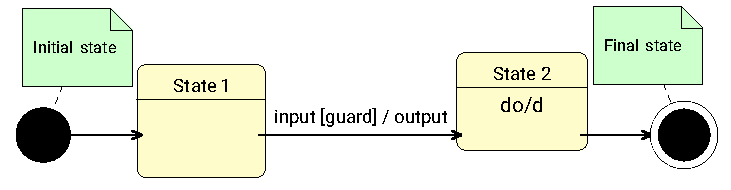
\includegraphics{bilder/State_Machine_Diagram.pdf}
    \caption{Beispiel für UML State Machine Diagram}
\end{figure}
% Kapitel 5
\clearpage
\section{Softwarearchitektur (Software Architecture)}
Softwarearchitektur umfasst:
\begin{itemize}
    \item Architekturcharakteristiken
    \item Architekturstyles (architecture styles, software system structure)
    \item Architekturentscheidungen
    \item Entwurfsmuster (design principles)
\end{itemize}
\begin{table}[ht]
    \centering
    \rowcolors{2}{\thepagecolor}{fgcolor!10!\thepagecolor}
    \resetrc{}
    \begin{tabular}{ll}
        \toprule
        \fatsf{Architekten}                                            & \fatsf{Entwicklungsteam}                    \\
        \midrule
        \fakebullet{}~\mlcell[l]{Die Charakteristiken der Architektur                                                \\aus der Abhängigkeitsanalyse zu ermitteln} & \fakebullet{}Klassenstruktur für jede Komponente erstellen \\
        \fakebullet{}Einen Architekturstil für das System auswählen    & \fakebullet{}UI(User Interface) entwerfen   \\
        \fakebullet{}Komponentenstruktur erstellen (über Klassenebene) & \fakebullet{}Quellcode schreiben und testen \\
        \bottomrule
    \end{tabular}
    \caption{Verantwortungsaufteilung bei der Softwarearchitektur}
    \label{tab:software_architecture_responsibilities}
\end{table}
\begin{figure}[ht]
    \centering
    \begin{tikzpicture}
        \node[draw,rounded corners,thick, minimum height=1cm,minimum width=3cm](n1){Architekten};
        \node[draw,rounded corners,thick, minimum height=1cm,minimum width=3cm,right=3cm of n1](n2){Entwicklungsteam};
        \draw[line width=2mm, draw=accentcolor,-triangle 45,postaction={draw, line width=4mm, shorten >=5mm, -}] (n1) -- node[line width= .4mm,pos=.4,text=white]{Input} (n2);
        \draw[-{Stealth},ultra thick](n1) to[out=90,in=90,looseness=.5] node[pos=.5,sloped,auto]{Adaption} (n2);
        \draw[{Stealth}-,ultra thick](n1) to[out=270,in=270,looseness=.5] node[pos=.5,sloped,below]{Rückmeldung(Feedback)} (n2);
    \end{tikzpicture}
    \caption{Relation Architekten-Entwickler}
\end{figure}
\clearpage
\subsection{Architekturcharakteristiken}
\begin{definition}[Architekturcharakteristik]\mbox{}
    \begin{itemize}
        \item Spezifiziert Operations-und Betriebskriterien um eine gewisse Anforderung zu implementieren
        \item Beeinflusst den Strukturentwurf, benötigt spezielle Architekturelemente (keine üblichen)
        \item Es ist nötig, dass die Anwendung wie gewünscht funktioniert (funktionale und nichtfunktionale Abhängigkeiten)
    \end{itemize}
\end{definition}
\fatsf{Operationscharakteristiken (Operational):}\begin{itemize}
    \item Verfügbarkeit (Availability): Zeitspanne, in der das System online/verfügbar ist
    \item Leistung (Performance): Umfasst Spitzenauslastungsanalysen, Antwortzeiten, Stresstests
    \item Skalierbarkeit: (Scalability): Fähigkeit auch mit einer steigenden Anzahl an Anfragen klarzukommen
\end{itemize}
\fatsf{Strukturell (Structural):}\begin{itemize}
    \item Erweiterbarkeit (Extensibility): Wie einfach es ist, neue Funktionalität hinzuzufügen
    \item Wartbarkeit (Maintainability): Wie einfach es ist, das System zu verbessern oder auszuwechseln (also zu warten)
    \item Wiederverwendbarkeit (Leveragability): Häufige Komponenten in mehreren Produkten wiederverwenden
    \item Lokalisierbarkeit (Localisation): Ünterstützung mehrerer Sprachen, Währungen, Einheiten, \dots
    \item Konfigurierbarkeit (Configuration): Möglichkeit für den Nutzer das System nach seinen Vorlieben durch eine benutzbare Oberfläche anzupassen.
\end{itemize}
\fatsf{Cross-Cutting (Divide and Conquer)}\begin{itemize}
    \item Barrierefreiheit: Muss auch nutzbar von Leuten mit Behinderung (Seh-, Höreinschränkungen, \dots) sein
    \item Datenschutz (Privacy): Möglichkeit, bestimmte Daten für andere Nutzer (auch priveligierte) unzugänglich zu machen
    \item Sicherheit (Security): Verschlüssellung, Authentifizierung, \dots
\end{itemize}
\subsection{Architekturstile}
\begin{itemize}
    \item Helfen die fundamentale Struktur eines Systems zu spezifizieren
    \item Haben einen großen Einfluss darauf, wie die fertige Architektur aussieht
    \item Definieren die globalen Eigenschaften des Systems (z.B. Wie Daten ausgetauscht werden können, welche Einschränkungen die Subsysteme haben)
\end{itemize}
Softwaresysteme sind normalerweise aus mehreren Architekturstilen zusammengesetzt
\clearpage
\subsubsection{Monolithische Architekturstile (Monolithic Architecture Styles)}
\paragraph{Ebenen (Layered)}\mbox{}\\
\begin{figure}[h]
    \centering
    \begin{tikzpicture}
        \node[rectangle split,rectangle split parts=4,draw,text centered, rectangle split part fill={red!30,blue!20, green!20, yellow!30}, rounded corners, thick] (A) {Presentationsebene (Presentation layer)\nodepart{two}Geschäftsebene (Business Layer)\nodepart{three}Beständigkeitsebene (Persistence Layer)\nodepart{four}Datenbankebene (Database Layer)};
    \end{tikzpicture}
\end{figure}
\FloatBarrier
\begin{itemize}
    \item Anzahl der Ebenen nicht festgelegt, manche Architekturen fassen Ebenen zusammen oder fügen neue hinzu
\end{itemize}

\begin{table}[ht]
    \centering
    \rowcolors{2}{\thepagecolor}{fgcolor!10!\thepagecolor}
    \resetrc{}
    \begin{tabular}{ll}
        \toprule
        \fatsf{pro}                                                  & \fatsf{contra}                                                      \\
        \midrule
        \fakebullet{}Simplizität                                     & \fakebullet{}Skalierbarkeit                                         \\
        \fakebullet{}Kosten                                          & \fakebullet{}Leistung (Parallelisierung \textbf{nicht} unterstützt) \\
        \fakebullet{}Architekturstil kann später ausgetauscht werden & \fakebullet{}Verfügbarkeit (lange startzeiten, \dots)               \\
        \fakebullet{}Gut für kleine-mittlere Anwendungen             &                                                                     \\ 
        \bottomrule
    \end{tabular}
    \caption{Layered-Architekturstil Pro Kontra}
    \label{tab:layered_style_pro_contra}
\end{table}

\paragraph{Model-View-Controller (MVC)}\mbox{}\\
Das MVC-Muster spaltet die Software in die fundamentalen Teile für interaktive Software auf:
\begin{itemize}
    \item Model: Enthält die Kernfunktionalität und Daten
          \begin{itemize}
              \item Unabhängig von dem Ausgabeformat und dem Eingabeverhalten
          \end{itemize}
    \item View: Präsentiert die Daten dem Nutzer
          \begin{itemize}
              \item Die Daten werden von dem Modell geladen
          \end{itemize}
    \item Controller: Verarbeitet die Eingaben des Nutzers
          \begin{itemize}
              \item Jeder View wird ein Controller zugewiesen
              \item Empfängt Eingaben (bspw. durch Events) und übersetzt diese für das Modell oder die Views
              \item Jede Interaktion geht durch den Controller
          \end{itemize}
\end{itemize}

\begin{figure}[ht]
    \centering
    \begin{tikzpicture}[->, every node/.style = { draw }]
        \node (controller) {Controller};
        \node [below left = 2 of controller] (view) {View};
        \node [below right = 2 of controller] (model) {Model};

        \draw (controller) -- (view);
        \draw (controller) -- (model);
        \draw (view) -- (model);
        \draw [dashed] (view) to[bend left] (controller);
        \draw [dashed, color = lightgray] (model) to[bend left] (view);
    \end{tikzpicture}
    \caption{Model-View-Controller}
    \label{fig:mvc}
\end{figure}
Controller und View sind direkt mit dem Modell gekoppelt, das Modell ist nicht direkt mit dem Controller oder der View gekoppelt (siehe \ref{fig:mvc}).
\clearpage
Nachteile:
\begin{itemize}
    \item Erhöhte Komplexität: Die Aufspaltung in View und Controller kann die Komplexität erhöhen ohne mehr Flexibilität zu gewinnen.
    \item Update Proliferation: Möglicherweise viele Updates; nicht alle Views sind immer an allen Änderungen interessiert.
    \item Kopplung View/Controller: View und Controller sind stark gekoppelt.
\end{itemize}
\subsubsection{Verteilte Architekturstile (Distributed Architecutral Styles)}
\paragraph{Dienstbasierend (Service-Based)}
\begin{itemize}
    \item Hauptvariante: \begin{itemize}
              \item Nur eine Bedienoberfläche (UI) für alle Services
              \item Services bestehen aus mehrenen Komponenten
              \item Alle Services greifen auf eine gemeinsame Datenbank zu
          \end{itemize}
    \item Nicht-Monolithische Variante (Non-Monolithic)\begin{itemize}
              \item Servicebasierende UIs (eine UI per service)
          \end{itemize}
    \item Servicelokale Datenbankvariante\begin{itemize}
              \item Services können eigene oder auch gemeinsame Datenbanken haben
          \end{itemize}
          \begin{figure}[ht]
              \centering
              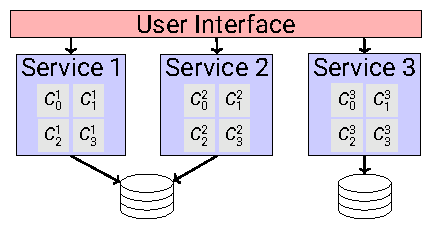
\includegraphics{bilder/service_local_service_based_architecture_style.pdf}
              \caption{Beispiel für Servislokale Datenbankvariante einer Dienstbasierenden Architektur}
          \end{figure}
\end{itemize}

%Kapitel 6
\clearpage
\section{Designprinzipien (Design Principles)}
\subsection{Softwarequalität}
\subsubsection{Faktoren}
Die Faktoren guter Software trennen sich in \textit{interne} und \textit{externe Faktoren}:
\begin{itemize}
    \item Interne Faktoren: Sicht der Entwickler (Code-Qualität). Stellt eine \enquote{White Box} dar.
    \item Externe Faktoren: Sicht der Nutzer (interne Qualitätsfaktoren sind nicht bekannt). Stellt eine \enquote{Black Box} dar.
\end{itemize}
\paragraph{Interne Faktoren}
\begin{itemize}
    \item Modularität
    \item Verständlichkeit
          \begin{itemize}
              \item Namensgebung (Methoden, Parameter, Variablen, \dots)
          \end{itemize}
    \item Kohäsion
    \item Prägnanz (keine/wenige Duplikate, klarer (kurzer) Code)
    \item \dots
\end{itemize}
% end

\paragraph{Externe Faktoren}
\begin{itemize}
    \item Korrektheit
    \item Verlässlichkeit
    \item Erweiterbarkeit
    \item Wiederverwendbarkeit
    \item Kompatibilität
    \item Portabilität
    \item Effizienz
    \item Nutzbarkeit
    \item Funktionalität
    \item Wartbarkeit
    \item \dots
\end{itemize}
\begin{defBox}
    \paragraph{Merkmale von Guter Software:}\begin{itemize}
        \item Wartbarkeit: Kann an Ansprüche des Kunden angepasst werden
        \item Effizienz: Keine Ressourcenverschwendung
        \item Usability: Muss für den Nutzer verständlich und benutzbar sein
        \item Verlässlichkeit (Dependability): Verursacht keinen wirtschaftlichen oder physikalischen Schaden falls das System fehlschlägt
    \end{itemize}
\end{defBox}

\clearpage
\subsection{Messen von Softwarequalität}
\subsubsection{Übersicht Metriken zum Messen von Softwarequalität}
\label{sec:metrics}

\begin{description}
    \item[Fan In] Anzahl Methoden, welche $ m $ aufrufen
    \item[Fan Out] Anzahl Methoden, welche $ m $ aufruft
    \item[Codelänge] Anzahl Zeilen
    \item[Zyklomatische Komplexität] Linear unabhängige Pfade durch den Code (Kontrollflussgraph)
    \item[Verschachtelungstiefe] Tiefe Verschachtelung von if/else, switch..case, etc. sind schwer zu verstehen
    \item[Gewichtete Methodenkomplexität pro Klasse] Gewichtete Summe der Methodenkomplexitäten
    \item[Vererbungstiefe] Tiefe Vererbungsbäume sind hochkomplex (Unterklassen)
\end{description}

\subsubsection{Zyklomatische Komplexität (Cyclomatic Complexity)}
Die Zyklomatische Komplexität $ C $ berechnet sich durch $ C = E - N + 2P $, wobei $ E $ die Anzahl der Kanten, $ N $ die Anzahl der Knoten und $ P $ die Anzahl der möglichen Zusammenhangskomponenten (in den meisten Fällen $ 1 $) des CFGs darstellt.

\subsubsection{Kontrollflussgraph (CFG)}
\label{diagram:cfg}

Ein Kontrollflussgraph stellt Code syntaxfrei dar, wodurch bessere Analysen möglich sind.

\paragraph{Beispiel}\mbox{}\\
Der in \figurename{} \ref{fig:fibonaccicodecfg} gezeigte Code wird in \figurename{} \ref{fig:cfg_example} als Kontrollflussgraph dargestellt.
\begin{figure}[ht]
    \centering
    %\begin{noindent}
    \begin{codeBlock}[autogobble]{}
        public static int fibonacci(final int num) {
        	if (num <= 0) {
        		throw new IllegalArgumentException();
        	}
        	int current = 1;
        	int previous = 0;
        	for (int i = 0; i < num - 1; i++) {
        		int next = current + previous;
        		previous = current;
        		current = next;
        	}
        	return current;
        }
	\end{codeBlock}
    %\end{noindent}
    \caption{Beispiel: Kontrollflussgraph / Code}
    \label{fig:fibonaccicodecfg}
\end{figure}
\begin{figure}[ht]
    \centering
    \begin{tikzpicture}[part/.style = { draw, align = center }]
        \node [part] (init) {init};
        \node [part, below = of init, label = 180:1] (step1) {\texttt{if (num <= 0)}};
        \coordinate [right = 6 of step1] (step1-);
        \node [part, below = of step1-, label = 180:11] (step1-1) {\texttt{throw new IllegalArgumentException();}};
        \node [part, below = of step1, label = 180:2,align = left] (step2) {\texttt{int current = 1;}\\\texttt{int previous = 0;}\\\texttt{int i = 0;}};
        %\node [part, below = of step2, label = 180:3] (step3) {\texttt{int previous = 0;}};
        \node [part, below = of step2, label = 180:3] (step4) {\texttt{for (; i < num - 1;)}};
        \coordinate [right = 5 of step4] (step4-);
        \node [part, below = of step4-, label = 180:31,align=left] (step4-1) {\texttt{int next = current + previous;}\\\texttt{previous = current;}\\\texttt{current = next;}};
        %\node [part, below = of step4-1, label = 180:32] (step4-2) {\texttt{previous = current;}};
        \node [part, below = of step4-1, label = 180:32] (step4-3) {\texttt{i++;}};
        \node [part, below = of step4, label = 180:4] (step5) {\texttt{return current;}};
        \node [part, below = of step5] (exit) {exit};

        \draw [->] (init) -- (step1);
        \draw [->] (step1) -| node [above] {\texttt{num <= 0}} (step1-1);
        \draw [->] (step1) -- node [left] {\texttt{num > 0}} (step2);
        \draw [->] (step2) -- (step4);
        %\draw [->] (step3) -- (step4);
        \draw [->] (step4) -| node [above] {\texttt{i < num - 1}} (step4-1);
        \draw [->] (step4-1) -- (step4-3);
        %\draw [->] (step4-2) -- (step4-3);
        \coordinate [right = 3.3 of step4-3] (back1);
        \coordinate (back2) at ([xshift=1cm,yshift=-1cm]step2.east);
        \draw (step4-3) -- (back1);
        \draw (back1) |- (back2);
        \draw [->] (back2) -- (step4);
        \draw [->] (step4) -- node [left] {\texttt{i >= num - 1}} (step5);
        \draw [->] (step5) -- (exit);
        \draw [->] (step1-1.south) |- ++(-4.3,-.5) |- (exit);
    \end{tikzpicture}
    \caption{Beispiel: Kontrollflussgraph}
    \label{fig:cfg_example}
\end{figure}
\FloatBarrier
\subsubsection{Heuristiken}
Design-Heuristiken helfen dabei, die Frage zu beantworten, ob das Design einer Software gut, schlecht oder irgendwo dazwischen ist.
\begin{itemize}
    \item Einsichten in OO-Design Verbesserungen
    \item Sprachunabhängig und erlauben das Einstufen der Integrität einer Software
    \item Nicht schwer aber schnell: Sollten Warnungen produzieren, welche unter anderem das ignorieren der selbigen erlauben wenn nötig
\end{itemize}

\textbf{Beispiel:} All Daten in einer Basisklasse sollten privat sein; die Nutzung von nicht-privaten Daten ist untersagt, es sollten Zugriffsmethoden erstellt werden, welche protected sind.
\clearpage
\subsubsection{Verknüpfen/Koppeln (Coupling)}

\begin{definition}[Class Coupling]
    ist ein Richtwert zur Messung der Abhängigkeiten zwischen Klassen und zwischen Paketen:
    \begin{itemize}
        \item  Eine Klasse C ist an Klasse D \textit{gekoppelt}, wenn C direkt oder indirekt von d abhängt
        \item  Eine Klasse, welche auf 2 anderen Klassen basiert, hat eine lockerere Kopplung als eine Klasse, welche auf 8 anderen Klassen basiert.
    \end{itemize}
\end{definition}

\paragraph{Kopplung in Java}\mbox{}\\
Die Klasse
%\begin{noindent}
\begin{codeBlock}[autogobble]{}
    import java.awt.event.ActionEvent;
    import java.awt.event.ActionListener;

    public class QuitAction implements ActionListener {
    	@Override
    	public void actionPerformed(ActionEvent event) {
    		System.exit(0);
    	}
    }
\end{codeBlock}
%\end{noindent}
ist mit den folgenden anderen Klassen gekoppelt: \texttt{ActionEvent}, \texttt{ActionListener}, \texttt{Override}, \texttt{System}, \texttt{Object}
% end
\paragraph{Lose Kopplung vs. Feste Kopplung}
\begin{itemize}
    \item Zu viele Verknüpfungen sind schlecht, denn:\begin{itemize}
              \item Änderungen in verknüpfter Klasse kann zu Dominoeffekt an Änderungen führen
              \item Eng verknüpfte Klassen sind isoliert betrachtet nur schwer zu verstehen
              \item Eng verknüpfte Klassen lassen sich nur schwer wiederverwenden (da alle Abhängigkeiten mit kopiert werden müssten)
          \end{itemize}
    \item Zu wenige bzw. gar keine Verknüpfungen sind aber auch unerwünscht, denn:\begin{itemize}
              \item Geht gegen das Prinzip der Objektorientierten Programmierung: "`Ein system von Verknüpften Objekten, die per Nachrichten Kommunizieren"'
              \item Führt zur Bildung von Gottklassen
              \item Führt zu hoher Komplexität
          \end{itemize}
    \item Generische Klassen müssen sehr wenige Verknüpfungen haben
    \item Viele Verknüpfungen von stabilen Bausteinen (Libraries, z.B. aus der Java-Standartbibliothek) ist kein Problem
\end{itemize}
\warning{Die Anforderung an lose Kopplung zur Wiederverwendbarkeit in (mystischen) Zukunftsprojekte birgt die Gefahr von unnötiger Komplexität und hohen Projektkosten!}
\clearpage
\subsubsection{Zuständigkeiten}
%\paragraph{Diagramm: Class-Responsibility-Collaborator-Karten (CRC-Karten)}\mbox{}\\
%\label{diagram:crc}

\paragraph{Beschreibung}\mbox{}\par
\begin{description}[leftmargin = 3cm]
    \item[Class] Der Name der Klasse/des Akteurs.
    \item[Responsibilities] Die Zuständigkeiten der Klasse; identifiziert die zu lösenden Probleme.
    \item[Collaborations] Andere Klassen/Akteure mit denen die Klasse/der Akteur kooperiert um eine Aufgabe zu erfüllen.
\end{description}
% end

%\todo{CRC-Karten: Beispiel}

\paragraph{Wichtige Konklusionen}\mbox{}\par
\begin{description}
    \item[Class]
          \begin{itemize}
              \item Der Name sollte deskriptiv und eindeutig sein.
          \end{itemize}
    \item[Responsibilities]
          \begin{itemize}
              \item Lange Zuständigkeitsliste  $ \implies $ Sollte die Klasse aufgeteilt werden?
              \item Zuständigkeiten sollten zusammenhängen.
          \end{itemize}
    \item[Collaborations]
          \begin{itemize}
              \item Viele Kollaboratoren $ \implies $ Sollte die Klasse aufgeteilt werden?
              \item \textbf{Vermeide zyklische Kollaboration!} $ \implies $ Es sollten höhere Abstraktionsebenen eingeführt werden.
          \end{itemize}
\end{description}

\subsubsection{Kohäsion(Cohesion)}
\begin{definition}[Kohäsion]
    ist ein Richtwert zur Messung des Zusammenhangs zwischen Elementen einer Klasse. Alle Operationen und Daten innerhalb einer Klassen sollten \enquote{natürlich} zu dem Konzept gehören, welches von der Klasse modelliert wird.
\end{definition}

Arten von Kohäsion (geordnet von sehr schlecht zu sehr gut):
\begin{enumerate}
    \item \textbf{Zufällig} (Coincidental, keine Kohäsion vorhanden): Kein sinnvoller Zusammenhang zwischen den Elementen einer Klasse (bspw. bei Utility-Klassen, \textbf{unerwünscht}).
    \item \textbf{Zeitliche Kohäsion}(Temporal): Alle Elemente einer Klasse werden \enquote{zusammen} ausgeführt.
    \item \textbf{Sequentielle Kohäsion}(sequential): Das Ergebnis einer Methode wird an die nächste übergeben.
    \item \textbf{Kommunikative Kohäsion} (Communicational): Alle Funktionen/Methoden einer Klasse lesen/schreiben auf der selben Eingabe/Ausgabe.
    \item \textbf{Funktionale Kohäsion}: Alle Elemente einer Klasse arbeiten zusammen zur Ausführung einer einzigen, wohldefinierten, Aufgabe. (\textbf{Idealfall})
\end{enumerate}

Klassen mit geringer Kohäsion sind zu vermeiden, da:
\begin{itemize}
    \item Schwer zu verstehen
    \item Schwer wiederzuverwenden
    \item Schwer wartbar (einfach änderbar)
    \item Symptomatisch für sehr grobkörnige Abstraktion
    \item Es wurden Aufgaben übernommen, die zu anderen Klassen delegiert werden sollten
\end{itemize}
Klassen mit hoher Kohäsion können oftmals mit einem einfachen Satz beschrieben werden.

\paragraph{Lack of Cohesion of Methods (LCOM)}\mbox{}\par
\begin{definition}[LCOM-Wert]
    Der \textit{Lack of Cohesion of Methods}-Wert (kurz LCOM-Wert) ist ein Richtwert zur Bewertung der Kohäsion einer Klasse.\\
    Sei $ C $ eine Klasse, $ F $ ihre Instanzvariablen und $ M $ ihre Methoden (Konstruktoren ausgenommen).\\
    Sei $ G = (M, E) $ ein ungerichteter Graph mit den Knoten $ V = M $ und den Kanten
    \[ E = \{ \langle m, n\rangle \in M \times M~|~\exists f \in F : (m \text{ nutzt } f) \land (n \text{ nutzt } f) \} \]
    dann ist $ \texttt{LCOM}(X) $ definiert als die Anzahl der zusammenhängenden Komponenten des Graphen $ G $.\\
    Ist $ n=\vert M \vert $ die Anzahl der Methoden, so gilt $ \texttt{LCOM}(X) \in [0, n] $.
\end{definition}


Ein hoher LCOM-Wert ist ein Indikator für zu geringe Kohäsion in der Klasse.

\subsection{Designprinzipien}
\subsubsection{Single-Responsibility-Principle (SRP)}
\begin{definition}[Single-Responsibility-Principle]
    \enquote{Eine Klasse sollte nur einen einzigen Grund haben, sich zu verändern},
    Also möglichst wenige Abhängigkeiten pro Klasse (ideal wäre nur eine), denn Abhängigkeiten sind der Hauptgrund für Änderungen
\end{definition}
\subsubsection{Inheritance vs. Delegation}
\begin{table}[ht]
    \centering
    \rowcolors{2}{\thepagecolor}{fgcolor!10!\thepagecolor}
    \resetrc{}
    \begin{tabular}{ll}
        \toprule
        \fatsf{Inheritance (Übernehmen/Erben)}                    & \fatsf{Delegation (Übergeben)}                                                 \\
        \midrule
        \fakebullet{}Auch irrelevante Funktionalität wird vererbt & \fakebullet{}~\mlcell[l]{Es wird ein Objekt übergeben, dass nur die gewünschte \\Funktionalität implementiert}\\
        \fakebullet{}Schwer zu Warten                             & \fakebullet{}Abhängigkeiten unverändert                                        \\
        \bottomrule
    \end{tabular}
    \caption{Inheritance vs Delegation}
    \label{tab:inheritance_vs_delegation}
\end{table}
\subsection{Kapselung(Encapsulation)}
\begin{definition}[Interface-Konzept]
    Ein Interface deklariert die Methodensignaturen und öffentlichen Konstanten seiner Subklassen
\end{definition}
\begin{itemize}
    \item Vorteile:\begin{itemize}
              \item Interfaces machen es Möglich, die Funktionalität von der Implementierung zu trennen
              \item Hilft dabei, ungerechtfertigte Vermutungen über die Implementierung zu vermeiden
              \item Interfaces sind stabiler als Implementierungen
              \item Um die Implementierung zu verändern, reicht es den Konstruktor zu verändern
              \item Einfacher um Kupplung zu vermeiden
          \end{itemize}
\end{itemize}
\clearpage
\subsubsection{Zugriffsrechte (Field Access)}
Angenommen es gäbe keine Zugriffsrechte und alles wäre Public, dann:
\begin{itemize}
    \item Verletzt das Prinzip der Informationsverbergung (information hiding principle):\begin{itemize}
              \item Keine Unterscheidung zwischen implementationsspezifischen und öffentlichen Daten
              \item Implementationsspezifische Details werden dem Client enthüllt
          \end{itemize}
    \item Instabiler Code, wenn die Implementation des Feldes sich ändert
    \item für Felder die als Argument oder unter einem Alias definiert sind ist es sehr schwer, die Abhängigkeiten zu erkennen
\end{itemize}
Also besser: Getter und Setter, sodass Zugriffe gezielt kontrolliert werden können
Probleme, wenn zu wenig freigegeben wird:\begin{itemize}
    \item Funktionalität muss ggf doppelt implementiert werden
    \item Verleitet einen dazu, die Abhängigkeiten falsch zu setzen
\end{itemize}
\warning{Instanzfelder (vom Konstruktor gesetzt) sollten niemals Public sein}
\subsection{Probleme}
\subsubsection{Gottklassen (God Classes)}%
\begin{wrapfigure}[5]{r}{.3\textwidth}%
    \vspace*{-5mm}
    
\includegraphics[width=5cm]{bilder/Godclass.pdf}
    %\caption{Gottklasse oder so}
\end{wrapfigure}
Eine Klasse kapselt einen Großteil oder alles der (Sub-) Systemlogik. Indikator von:
\begin{itemize}
    \item Schlecht verteilter Systemintelligenz
    \item Schlechtem OO-Design, welches auf der Idee von zusammenarbeitenden Objekten aufbaut
\end{itemize}

\paragraph{Lösungsansätze}\mbox{}\par
\begin{itemize}
    \item Gleichmäßige Verteilung der Systemintelligenz. \\
          Oberklassen sollten die Arbeiten so gleich wie möglich verteilen.
    \item Vermeidung von nichtkommunikativen Klassen (mit geringer Kohäsion). \\
          Klassen mit geringer Kohäsion arbeiten oftmals auf einem eingeschränkten Teil der eigenen Daten und haben großes Potential, Gottklassen zu werden.
    \item Sorgfältige Deklaration und Nutzung von Zugriffsmethoden. \\
          Klassen mit vielen (öffentlichen) Zugriffsmethoden geben viele Daten nach außen und halten somit das Verhalten nicht an einem Punkt.
\end{itemize}
% end
% end

\subsubsection{Class Proliferation}
Zu viele Klassen in Relation zu der Größe des Problems. Oftmals ausgelöst durch zu frühes Ermöglichen von (mystischen) zukünftigen Erweiterungen.

\clearpage
\section{Designtechniken}
\subsection{Dokumentation}
\subsubsection{Lesbarkeit}\begin{itemize}
    \item Zu einer guten Lesbarkeit gehören:\begin{itemize}
              \item Dokumentation
              \item Kommentare im Quellcode
              \item der Quellcode selber:\begin{itemize}
                        \item Codestilkonventionen
                        \item Einschränkungen der Nutzung bestimmter Sprachkonstrukte (z.B. var in Java)
                        \item gute Benennung von Klassen, Methoden und Variablen
                        \item aussagekräftige Kommentare
                    \end{itemize}
          \end{itemize}
\end{itemize}
\subsubsection{Arten von Kommentaren}
\begin{itemize}
    \item API-Kommentare:\begin{itemize}
              \item Ausführliche Klassen-und Methodenlevelkommentare
              \item Zielgruppe: Andere Entwickler, die den Code als Library/Framework nutzen
              \item Muss enthalten:\begin{itemize}
                        \item Einschränkungen von Methodenparametern über den Typ hinaus (z.B. nicht null oder nicht negativ)
                        \item Auswirkungen auf den Zustand des Objektes
                        \item Wann und welche Exceptions geworfen werden
                    \end{itemize}
          \end{itemize}
    \item Statement-Level-Comments:\begin{itemize}
              \item Kommentare darüber, warum welche Befehle innerhalb einer Methode genutzt wurden
              \item Zweck: Implementation beschreiben, Code strukturieren
              \item Zielgruppe: Entwickler, die an dem selben Projekt mitarbeiten
              \item Sollte nur genutzt werden, wenn auch wirklich nötig
              \item Kann ein Indikator für sehr Komplexen Code sein $\Rightarrow$ Überarbeiten (refactor)
          \end{itemize}
\end{itemize}

\clearpage
\subsection{Überarbeiten (Refactoring)}
\begin{definition}[Refactoring]
    ist eine disziplinierte Technik, um einen existierenden Codekörper umzustrukturieren, und dabei seine interne Struktur zu verändern, ohne die Verhaltensweise nach außen hin zu verändern.
\end{definition}
\paragraph{Ziele:}\begin{itemize}
    \item Hinzufügen von neuen Funktionen vorbereiten
    \item Design verbessern, z.B. Kohäsion verbessern
    \item Verständlichkeit verbessern
    \item Wartbarkeit verbessern
\end{itemize}
\subsubsection{Gründe für das Überarbeiten}
\begin{itemize}
    \item Macht das Hinzufügen neuer Funktionen einfacher
    \item Weniger redundanter Code
    \item Vermeiden von verschachtelten Bedingungen
    \item Macht Code einfacher/verständlicher
\end{itemize}
\subsubsection{Methode Extrahieren (Extract Method)}
\begin{itemize}
    \item Wann?: \begin{itemize}
              \item wenn eine Methode zu viele Dinge macht
              \item wenn eine Funktionalität mehrfach innerhalb einer Methode oder von mehreren Methoden gebraucht wird
          \end{itemize}
    \item Vorgehensweise:\begin{enumerate}
              \item Neue Methode erstellen (Target)
              \item Extrahierten Code zur neuen Methode kopieren
              \item Lokale Variablen identifizieren, die in dem extrahierten Code verwendet wurden und als Parameter übergeben
              \item Code in ursprünglicher Methode mit Methodenaufruf ersetzen
          \end{enumerate}
\end{itemize}
\clearpage
\subsubsection{Methode Verschieben (Move Method)}
\begin{itemize}
    \item Wann:\begin{itemize}
              \item Methode nutzt keine anderen Funktionen ihrer Klasse,
              \item Methode überschreibt keine andere Methode oder wird überschrieben \textbf{und}
              \item Methode berechnet etwas für ein anderes Objekt
          \end{itemize}
          \begin{itemize}
              \item Vorgehensweise:\begin{enumerate}
                        \item Methode in Zielklasse deklarieren
                        \item Methode in Zielklasse kopieren und anpassen
                        \item Herausfinden, wie die Zielklasse am Besten referenziert werden kann
                        \item Quellmethode zu Delegationsmethode umwandeln (Logik findet in Zielklasse statt, aber Aufruf in Quellklasse)
                        \item Entscheiden, ob die Quellmethode noch gebraucht wird, oder ob der Aufruf in der Zielklasse sinvoller ist
                    \end{enumerate}
          \end{itemize}
\end{itemize}
\subsubsection{Klasse Extrahieren (Extract Class)}
\begin{itemize}
    \item Wann:\begin{itemize}
              \item Klasse hat zwei oder mehr unabhängige Abhängigkeiten
              \item Keine andere Klasse ist für Move Method geeignet
          \end{itemize}
    \item Vorgehensweise\begin{enumerate}
              \item Neue Klasse erstellen
              \item Neue Klasse als Attribut der alten Klasse
              \item Move Method der Methode
              \item Abhängigkeiten erneut prüfen
          \end{enumerate}
\end{itemize}

\subsection{Idiome}
Idiome sind \textit{keine} Entwurfsmuster, sondern kleine Codeschnipsel:
\begin{itemize}
    \item Limitiert in der Größe und
    \item oftmals spezifisch für eine Programmiersprache.
\end{itemize}
% end


\clearpage
\section{Entwurfskonzepte (Design Patterns)}
\begin{definition}[Design Pattern]\mbox{}
    \begin{itemize}
        \item beschreibt ein Problem, welches öfters innerhalb der Domäne auftritt
        \item bietet Bauplan für Lösung des Problemes, welcher oft wiederverwendet werden kann, aber niemals den Bauplan selbst sondern eine angepasste Form
    \end{itemize}
\end{definition}
\begin{itemize}
    \item Dokumentiertes Expertenwissen
    \item Nutzung von generischen Lösungen
    \item Erhöhung des Abstraktionsgrades
    \item Ein Muster hat einen Namen
    \item Die Lösung kann einfach auf andere Varianten des Problems angewandt werden
\end{itemize}
\paragraph{Aufbau eines Patterns}\begin{description}
    \item[Pattern Name] Kurzer, deskriptiver Name
    \item[Problembeschreibung] \begin{itemize}
              \item Wann das Pattern angewandt werden soll
              \item Fälle, für die das Pattern eine Lösung bietet
          \end{itemize}
    \item[Lösung] \begin{itemize}
              \item Elemente, die das Design beschreiben
              \item Relationen, Abhängigkeiten, Zusammenhänge
          \end{itemize}
    \item[Konzequenzen] \begin{itemize}
              \item Nebenwirkungen, Einschränkungen, Auswirkungen auf Flexibilität, Erweiterbarkeit und Portabilität
          \end{itemize}
\end{description}
\paragraph{Vorlage Design Pattern}\mbox{}\\
\begin{table}[ht]
    \centering
    \rowcolors{2}{\thepagecolor}{fgcolor!10!\thepagecolor}
    \resetrc{}
    \begin{tabular}{l}
        \toprule
        1.\quad\mlcell[l]{
        \fakebullet{}\textbf{Name}: Name des Patterns                                                     \\
            \fakebullet{}\textbf{Absicht}: Ziele und Gründe warum man das Pattern verwenden sollte
        }                                                                                                 \\
        \midrule
        2.\quad\mlcell[l]{
        \fakebullet{}\textbf{Motivation}: Problemsituation beschreiben (Szenario)                         \\
            \fakebullet{}\textbf{Anwendbarkeit}: Bedingungen, wann man es anwenden kann
        }                                                                                                 \\
        \midrule
        3.\quad\mlcell[l]{
        \fakebullet{}\textbf{Struktur}: statische Struktur des Patterns (z.B. UML Klassendiagramm)        \\
        \fakebullet{}\textbf{Participants}(Teilnehmer): Welche Klassen sind beteiligt                     \\
        \fakebullet{}\textbf{Collaboration}: Zusammenspiel der Teilnehmer                                 \\
            \fakebullet{}\textbf{Implementation}: Wie das Pattern angepasst/implementiert werden kann
        }                                                                                                 \\
        \midrule
        4.\quad\mlcell[l]{
        \fakebullet{}\textbf{Konzequenzen}: Nebenwirkungen, Einschränkungen,                              \\
            Auswirkungen auf Flexibilität, Erweiterbarkeit und Portabilität
        }                                                                                                 \\
        \midrule
        5.\quad\mlcell[l]{
        \fakebullet{}\textbf{Bekannte Anwendungsfälle}: Beispiele, wann das Pattern verwendet werden soll \\
            \fakebullet{}\textbf{Verwandte Patterns}: Referenzen und Vergleiche mit anderen Patterns
        }                                                                                                 \\
        \bottomrule
    \end{tabular}
    \caption{Vorlage Design Pattern}
    \label{tab:design_pattern_template}
\end{table}
\clearpage
\subsection{Einführung}


\subsubsection{Template Method}
\begin{definition}[Template Method]
    Die Template-Methode definiert den Algorithmus unter Nutzung von abstrakten (und konkreten) Operationen.
\end{definition}
\paragraph{Kurzfassung}\mbox{}\\
\textbf{Ziel:} Implementierung eines Algorithmus, welcher erlaubt ihn auf mehrere spezifische Probleme anzuwenden.

\textbf{Idee:} Es wird ein Algorithmus implementiert, welcher konkrete Aktionen an abstrakte Methoden und damit Unterklassen weiterreicht.

\textbf{Konsequenzen:}
\begin{itemize}
    \item Aufteilung von variablen und statischen Teilen
    \item Verhinderung von Codeduplikation in Unterklassen
    \item Kontrolle über Erweiterungen von Unterklassen
\end{itemize}
% end

\paragraph{Generisches Klassendiagramm}\mbox{}\\
\begin{figure}[ht]
    \centering
    \begin{tikzpicture}
        \umlclass{AbstractClass}{}{
            + templateMethod() \\
            \umlvirt{opA()} \\
            \umlvirt{opB()} \\
            \dots \\
        }
        \umlclass[right = 1 of AbstractClass]{ConcreteClass}{}{
            opA() \\
            opB() \\
            \dots \\
        }

        \umlinherit{ConcreteClass}{AbstractClass}
        \umlnote[width = 3.5cm, left = 1 of AbstractClass]{AbstractClass}{\texttt{templateMethod() \{} \\ \texttt{ opA();} \\ \texttt{ \dots} \\ \texttt{ opB();} \\ \texttt{\}}}
    \end{tikzpicture}
    \caption{UML: Template Method Pattern}
\end{figure}
% end

\paragraph{Varianten/Erweiterungen}\mbox{}\\
Statt abstrakten Operationen, welche implementiert werden \textit{müssen}, können Hooks verwendet werden, welche implementiert werden \textit{können}.
% end
% end

\clearpage
\subsubsection{Strategy}
\paragraph{Kurzfassung}\mbox{}\\
\textbf{Motivation:}
\begin{itemize}
    \item Viele verwandte Klassen unterscheiden sich ausschließlich in ihrem Verhalten statt unterschiedlich verwandte Abstraktionen zu implementieren
\end{itemize}

\textbf{Ziel:}
\begin{itemize}
    \item Erlaubt das Konfigurieren einer Klasse mit einem von vielen Verhaltensvarianten
    \item Implementierung unterschiedlicher Algorithmusvarianten können in der Klassenhierarchie verbaut werden
\end{itemize}

\textbf{Idee:} Definition einer Familie von Algorithmen, Kapselung von jedem und herstellen einer Austauschbarkeit.

\textbf{Konsequenzen:}
\begin{itemize}
    \item Nutzer muss sich im klaren darüber sein, wie sich die Implementierungen unterscheiden und sich für eine entscheiden
    \item Nutzer sind Implementierungsfehlern ausgesetzt
    \item Strategy sollte nur genutzt werden, wenn das konkrete Verhalten relevant für den Nutzer ist
\end{itemize}
% end

\paragraph{Generisches Klassendiagramm}\mbox{}\\
\begin{figure}[ht]
    \centering
    \begin{tikzpicture}
        \umlinterface{Strategy}{}{
            \umlvirt{+ stategyOperation()} \\
        }
        \umlclass[below = 2 of Strategy]{ConcreteStrategyB}{}{
            + stategyOperation() \\
        }
        \umlclass[left = 1 of ConcreteStrategyB]{ConcreteStrategyA}{}{
            + stategyOperation() \\
        }
        \umlclass[right = 1 of ConcreteStrategyB]{ConcreteStrategyC}{}{
            + stategyOperation() \\
        }
        \umlsimpleclass[left = 3 of Strategy]{Context}

        \umlinherit[geometry = |-|]{ConcreteStrategyA}{Strategy}
        \umlinherit{ConcreteStrategyB}{Strategy}
        \umlinherit[geometry = |-|]{ConcreteStrategyC}{Strategy}
        \umluniassoc{Context}{Strategy}
    \end{tikzpicture}
    \caption{UML: Stategy Pattern}
\end{figure}
% end

\paragraph{Beschreibung}\mbox{}\\
Der Context (Nutzer) erstellt Instanzen von konkreten Strategien, welche den Algorithmus in einem Interface definieren.
% end

\paragraph{Varianten/Erweiterungen}\mbox{}\par
\begin{itemize}
    \item Optionale Strategy-Objekt
          \begin{itemize}
              \item Context prüft, ob Strategy-Objekt gesetzt wurde und nutzt es entsprechend
              \item Vorteil: Nutzer sind nur dem Strategy-Objekt ausgesetzt, wenn das Standardverhalten nicht genutzt werden soll
          \end{itemize}
\end{itemize}
% end
% end

\subsubsection{Observer}
\paragraph{Kurzfassung}\mbox{}\\
\textbf{Motivation:} OOP (Objektorientierte Programmierung) vereinfacht die Implementierung einzelner Objekte, die Verdrahtung dieser kann allerdings schwer sein, sofern man die Objekte nicht hart koppeln möchte.

\textbf{Ziel:} Entkopplung des Datenmodells (Subjekt) von den Stellen, welche an Änderungen des Zustands interessiert sind. Voraussetzungen:
\begin{itemize}
    \item Das Subjekt sollte nichts über die Observer wissen.
    \item Identität und Anzahl der Observer ist nicht vorher bekannt.
    \item Neue Observer sollen dem System später hinzugefügt werden können.
    \item Polling soll vermieden werden (da inperformant).
\end{itemize}

\textbf{Idee:} Erstellung von Observern (generalisiert mittels eines Interfaces), welche einem Subjekt hinzugefügt werden können und aufgerufen werden können.

\paragraph{Generisches Klassendiagramm}\mbox{}\\
\begin{figure}[ht]
    \centering
    \begin{tikzpicture}
        \umlclass[type = abstract, x = 0, y = 0]{Subject}{}{
            + attach(Observer) \\
            + detach(Observer) \\
            \# notify() \\
        }
        \umlinterface[x = 7, y = 0]{Observer}{}{
            \umlvirt{+ update(\dots)} \\
        }
        \umlclass[x = 0, y = -4]{ConcreteSubject}{}{
            + getState() \\
            + modifyState() \\
        }
        \umlclass[x = 7, y = -4]{ConcreteObserver}{}{
            + update(\dots) \\
        }

        \umlinherit{ConcreteSubject}{Subject}
        \umlinherit{ConcreteObserver}{Observer}
        \umluniassoc[mult2 = *]{Subject}{Observer}
        \umluniassoc[stereo = optional]{ConcreteObserver}{ConcreteSubject}
    \end{tikzpicture}
    \caption{UML: Observer Pattern}
\end{figure}
% end

\paragraph{Beschreibung}\mbox{}\par
\begin{description}
    \item[Subject] Abstrakte Klasse, bietet Methoden zur Implementierung des Musters an.
    \item[Observer] Interface zum Empfangen von Signalen eines Subjekts.
    \item[ConcreteSubject] Das konkrete Subjekt, sendet Benachrichtigungen an die Observer
    \item[ConcreteObserver] Ein konkreter Observer (implementiert Observer Interface), registriert sich beim Subjekt, empfängt Nachrichten vom Subjekt
\end{description}
% end

\clearpage
\textbf{Konsequenzen:}
\begin{itemize}
    \item Vorteile
          \begin{itemize}
              \item Abstrakte Kopplung zwischen Subjekt und Observer
              \item Unterstützung von Broadcast-Kommunikation
          \end{itemize}
    \item Nachteile
          \begin{itemize}
              \item Risiko von Update-Kaskaden zwischen Subjekt, Observer und dessen Observern
              \item Updates werden an alle gesendet, sind aber nur für einige relevant
              \item Fehlende Details über die Änderungen (Observer muss dies selbst herausfinden)
              \item Generelles Interface für Observer schränkt die Parameter stark ein
          \end{itemize}
\end{itemize}
% end

\paragraph{Varianten/Erweiterungen}\mbox{}\par
\begin{itemize}
    \item Pull Mode:\begin{itemize}
              \item Subjekt wird nach Änderung gefragt
              \item Führt oft dazu, dass nicht nur die Änderung sondern mehr Daten abgerufen werden müssen
          \end{itemize}
    \item Push Mode:\begin{itemize}
              \item Der update() Methode wird die Änderung als Parameter übergeben
              \item Nur der Bereich der auch wirklich geändert werden muss wird geändert $\Rightarrow$ bessere Antwortzeiten
              \item Erfordert genaues Wissen dessen, was geupdated werden muss, also Fehleranfälliger
          \end{itemize}
\end{itemize}

\clearpage
\subsubsection{Fabrikmethode (Factory Method)}
\begin{definition}[Factory Method]
    Deklariert ein Interface für Objekterstellung, aber lässt die Subklassen selbst entscheiden, welche Klasse instanziert werden soll (z.B. \texttt{public abstract Document createDocument()} und Klasse kann z.B. Textdokument oder ander Ableitung dafür nutzen)
\end{definition}
\begin{figure}[ht]
    \centering
    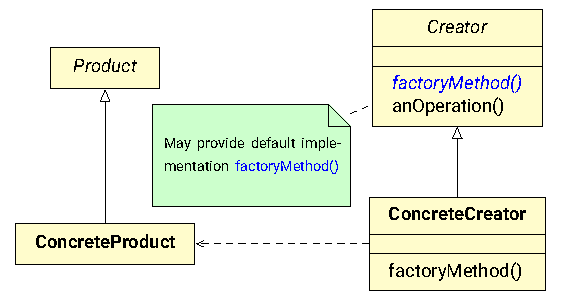
\includegraphics[width=.5\textwidth]{bilder/factory_method_pattern.pdf}
    \caption{Pattern Structure Factory Method}
\end{figure}
\FloatBarrier
\begin{description}
    \item[Product] Interface für Objekte, die von der factory Methode erstellt werden
    \item[Konkretes Produkt] Implementiert das Produkt-Interface
    \item[Generator (Creator)] \begin{itemize}
              \item Deklariert die Factory-Methode die ein Objekt des Types Product erstellt
              \item Generator kann default Implementierung der Factory-Methode enthalten, die ein Konkretes Produkt erstellt
          \end{itemize}
    \item[Konkreter Generator] Überschreibt die Factory-Methode, sodass diese ein anderes Konkretes Produkt erstellt
\end{description}
\paragraph{Konzequenzen}
\begin{itemize}
    \item Der Client-Code kennt nur das Produkt-Interface
    \item Stellt einen Hook für Superklassen bereit
\end{itemize}
\paragraph{Varianten}
\begin{itemize}
    \item Generator als Abstrakte Klasse
    \item Generator als Konkrete Klasse, mit einer sinvollen default-Implementierung
\end{itemize}
\clearpage
\subsubsection{Abstrakte Fabrik (Abstract Factory)}
\begin{figure}[ht]
    \centering
    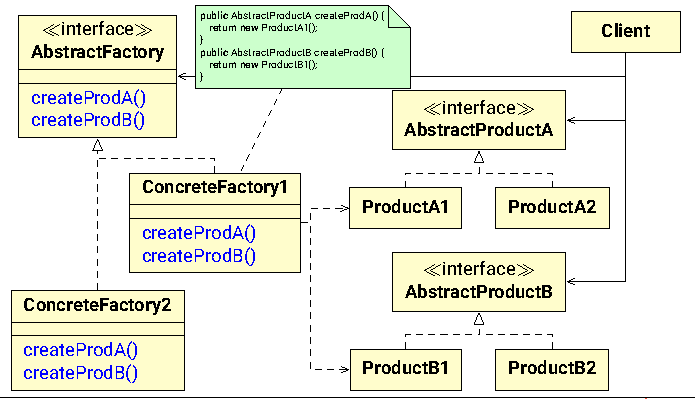
\includegraphics[width=.7\textwidth]{bilder/SE_08_DesignPatterns-seiten-37_cropped.pdf}
    \caption{Abstrakte Fabrik- Pattern structure}
\end{figure}
\FloatBarrier
\begin{description}
    \item[Abstrakte Fabrik] Stellt Interface für die Produkterstellung einer Familie bereit
    \item[Konkrete Fabrik] Implementiert Operationen um Konkrete Produkte zu erstellen
    \item[Abstraktes Produkt] Deklariert ein Interface um die Konkreten Produkte zu erstellen
    \item[Konkretes Produkt] Stellt Implementation für das Produkt, welche von der Konkoreten Fabrik erstellt wurde bereit
    \item[Client] Erstellt Produkt indem die Konkrete Fabrik genutzt wird, dabei wird das Abstrakte Produkt Interface implementiert
\end{description}
\begin{itemize}
    \item \textbf{Vorteile:}\begin{itemize}
              \item Code muss nicht über alle Konkreten Produkte bescheid wissen
              \item Eine Zeile Code zu verändern reicht aus, um andere Produkte zu unterstützen
              \item Kann mehrere Produkte unterstützen
              \item Erzwingt die Erstellung von konsistenten Produktfamilien
          \end{itemize}
    \item \textbf{Nachteile:}\begin{itemize}
              \item Code muss einer neuen Konvention zur Erstellung von Produktfamilien folgen (Statt den Standardkonstruktor zu nutzen)
          \end{itemize}
\end{itemize}

\clearpage
\section{Verifikation (Verification)}
\subsection{Einführung}

\subsection{Verifikation und Validierung}
\begin{definition}[Verifikation]
    Wird das System korrekt erstellt?
\end{definition}
\begin{definition}[Validierung]
    Wird das richtige System erstellt?
\end{definition}

\subsubsection{Techniken}
\paragraph{Statische Techniken}\mbox{}\\
Statische Techniken erfordern nicht, dass das Programm ausgeführt wird.

\begin{description}
    \item[Software Reviews] Händische/Manuelle Überprüfung
    \item[Automatisierte Statische Analyse] Softwareanalyse, bspw. Typprüfer
    \item[Formale Verifikation] Formaler Beweis, dass ein Programm eine bestimme Eigenschaft erfüllt
\end{description}

Siehe \ref{sec:metrics}.
% end

\paragraph{Dynamische Techniken}\mbox{}\\
Dynamische Techniken erfordern, dass das Programm ausgeführt wird.

\begin{description}
    \item[Testen] Führt das Programm aus und testet es auf bestimmte Eigenschaften (Verhalten)
    \item[Laufzeitüberprüfung] Analysetools, welche Programme auf Einhaltung bestimmter Einschränkungen (bspw. Speichereinschränkungen) testen
\end{description}
% end
% end

\clearpage
\subsubsection{Codeuntersuchung (Code reviews)}
\begin{definition}[Code Review]
    die Codeuntersuchung ist ein strukturierter Inspektionsprozess einer Software,
    der meist im Team ausgeführt wird, mit dem Ziel mögliche Fehler im Code zu finden.
\end{definition}
Das Ziel der Codeuntersuchung, ist
\begin{itemize}
    \item Programmfehler,
    \item Standardfehler und
    \item Designfehler
\end{itemize}
zu finden.

Dies wird üblicherweise in (externen) Teams ausgearbeitet, welche den Code systematisch analysieren.

Eine mögliche Checkliste ist bspw.:
\begin{description}
    \item[Dokumentation] Ist der Code sinnvoll, verständlich und ausreichend Dokumentiert?
    \item[Verständlichkeit] Ist der Code verständlich und die Variabeln sinnvoll benannt?
    \item[Struktur] Werden alle Programmierstandards eingehalten und erfüllt der Code das vereinbarte Design?
    \item[Fehlerbehandlung] Sind die am häufigsten vorkommenden Fälle abgedeckt?
    \item[Defensive Programmierung] Werden alle Dateien und Geräte im Fehlerfall in einem validen Status hinterlassen? 
            Sind die Sichtbarkeiten für die Klassen, Methoden und Felder so restriktiv wie möglich gewählt?
\end{description}

\begin{itemize}
    \item Vorteile: \begin{itemize}
              \item Studien zeigen, dass es funktioniert und Kosten sparen kann
              \item Helfen dabei, Wissen über den Code bei den Teammitgliedern zu verteilen
              \item Fehler können gefunden werden, bevor sie in Tests auftauchen
              \item Können Codequalität erhöhen
              \item Keine Codeausführung nötig
          \end{itemize}
    \item Nachteile\begin{itemize}
              \item Erfordert \enquote{Erwachsene} Herangehensweise: Teammitglieder können sich kritisiert fühlen
              \item Unter Zeitdruck fühlen sie sich unproduktiv an
              \item Funktionieren nur gut wenn korrekt geführt
          \end{itemize}
\end{itemize}
% end
% end
\clearpage
\subsection{Testen}
\begin{defBox}
    \enquote{Programmtesten kann zwar die Existenz von Fehlern aufzeigen, aber niemals ihre Abwesenheit beweisen!}\mbox{}\\\mbox{}\hfill — E. W. Dijkstra, EWD 249
\end{defBox}
\begin{definition}[Testplan]
    Ein \textit{Testplan} ist zur Ausführung durch Menschen gedacht. Er dokumentiert die Schritte des Tests und das jeweilige erwartete Ergebnis. In der Testausführung kann das eigentliche Ergebnis dann mit dem Erwarteten verglichen werden.
\end{definition}

\begin{definition}[Testfall (Test case)]
    besteht aus\begin{itemize}
        \item Startzustand (Pretest state)
        \item Testlogik
        \item Erwarteten Ergebnissen
    \end{itemize}
\end{definition}
\begin{definition}[Test Suite]
    Eine Sammlung an Testfällen heißt Test Suite (Testsammlung)
\end{definition}
\begin{definition}[Test Run]
    Ausführung einer Test Suite auf der IUT, wenn der Test durch geht kriegt er den \enquote{Verdict Pass} (Urteilspass), sonst bezeichnet man ihn als gescheitert (failed).
\end{definition}
\begin{definition}[Test Driver (Treiber)]
    Klasse oder Programm, welches den Test auf die IUT anwendet
\end{definition}
\begin{definition}[Test Harness (Gerüst)]
    System von Testtreibern und anderen Tools, um die Testausführung zu unterstützen
\end{definition}
% end

\subsubsection{Testtypen}
\paragraph{Unit Tests}\mbox{}\\
Sehr kleine, automatisierte, Tests, welche eine Funktionalität testen. In typischen Softwareprojekten finden sich $ \leq 1000 $ Unit Tests.
% end

\paragraph{Integrations-Tests}\mbox{}\\
Testen eines kompletten (Unter-) Systems, um die Zusammenarbeit der Komponenten zu testen.
% end

\paragraph{Systemtests}\mbox{}\\
Testen einer komplett integrierten Applikation (Funktion, Performanz, Stresstest, \dots).
% end
% end
\clearpage


\subsection{Testabdeckung}
\begin{definition}[Bedingung]
    Eine \textit{Bedingung} ist \texttt{ein} boolescher Audruck.
\end{definition}
\begin{definition}[Entscheidung]
    Eine \textit{Entscheidung} ist eine Zusammensetzung von Bedingungen, welche bspw. den Test eines \texttt{if}-Ausdruckes darstellt.
\end{definition}
\begin{definition}[Basisblock (Basic block)]
    Ein Basisblock $B$ ist eine maximale Sequenz von Instruktionen ohne Sprünge.
\end{definition}
\subsubsection{Strukturell}
Strukturelle Testabdeckung basiert auf dem Kontrollflussgraphen (CFG) eines Programms\begin{itemize}
    \item Statement Coverage (SC): Alle Ausdrücke wurden mindestens einmal ausgeführt.
    \item Basic Block Coverage (BBC): Alle Basisblöcke wurden mindestens einmal ausgeführt.
    \item Branch Coverage (BC): Jede Seite von jedem Knoten wurde mindestens einmal ausgeführt (d.h. jede Kante eines Kontrollflussgraphen).
    \item Path Coverage (PC): Alle Pfade wurden mindestens einmal ausgeführt (siehe CFG).
\end{itemize}

\subsubsection{Logisch}\begin{itemize}
    \item Condition Coverage (CC): Jede Bedingung wurde mindestens einmal zu wahr und falsch ausgewertet.
    \item Decision Coverage (DC): Jede Entscheidung wurde mindestens einmal zu wahr falsch ausgewertet.
    \item Modified Condition Decision Coverage (MCDC): Kombiniert Aspekte der Condition Coverage, Decision Coverage und Unabhängigkeitstests.\\
          Ein Test für eine Bedingung $ c $ in Entscheidung $ d $ (Duplikate von $ c $ werden nicht gezählt) erfüllt MCDC gdw.
          \begin{itemize}
              \item er $ d $ mindestens zweimal auswertet,
              \item davon $ c $ einmal zu wahr und einmal zu falsch auswertet,
              \item $ d $ in beiden Fällen unterschiedlich ausgewertet wird und
              \item die anderen Bedingungen in $ d $ in beiden identisch oder in mindestens einem nicht ausgewertet werden.
          \end{itemize}
          Für 100\%-ige MCDC-Abdeckung muss dies für jede Bedingung in dem Programm gelten.
    \item Multiple-Condition Coverage (MCC): Alle möglichen Kombinationen innerhalb einer Entscheidung wurden mindestens einmal ausgeführt.
\end{itemize}
\clearpage
\subsection{Testautomation}
Ein Testautomationssystem
\begin{itemize}
    \item startet die \enquote{implementation under test} (IUT),
    \item setzt die Umgebung auf,
    \item bringt das System in den erwarteten Ausgangszustand,
    \item wendet die Testdaten an und
    \item evaluiert die Ergebnisse und den Zustand des Systems.
\end{itemize}
\subsubsection{Automatisierte Test Case Generierung (ATCG)}
\paragraph{White Box}\begin{itemize}
    \item Syntaktischer Ansatz: Suchen nach Bedingungen, Evaluierung ermöglicht Logic-Based Coverage
    \item Unerreichbarer Code kann gefunden werden
    \item Symbolische Ausführung: versuchen, CFG mit verschiedensten Werten durchzulaufen, Evaluierung ermöglicht Structural Coverage
\end{itemize}
\vspace*{-1ex}
\paragraph{Black Box}\begin{itemize}
    \item Analyse der Ein-und Ausgabedaten der IUT
    \item Probleme: Library Calls, unnötige Testfälle, Rekursion, \dots
\end{itemize}
\vspace*{-1ex}
\paragraph{Test Coverage Recording}\begin{enumerate}
    \item IUT initialisieren
    \item Test Suite ausführen und Informationen während des Testlaufes sammeln
    \item Test Coverage analysieren und darstellen
\end{enumerate}
\vspace*{-1ex}
\paragraph{Test Oracle Synthesis}\begin{itemize}
    \item Menschliches Orakel: Zeitaufwändig und Fehleranfällig
    \item Testen durch Code: Braucht Expertenwissen, schwer zu warten
\end{itemize}
\vspace*{-1ex}
\paragraph{Static Checking}
Basiert auf CFG, hilft bei:
\begin{itemize}
    \item Runtime Exceptions, Informationsfluss
    \item Vollautomatisiert
    \item Gefahr: False Positives
    \item Zeitaufwand gering
\end{itemize}
\vspace*{-1ex}
\paragraph{Dynamic Checking}\begin{itemize}
    \item Runtime Monitoring
\end{itemize}
\vspace*{-1ex}
\paragraph{Formal Checking}\begin{itemize}
    \item Design-By-Contract (wie Racket Verträge mit precoditions und so)
\end{itemize}
% end
% end
% end
% end
% end

\clearpage
\section{Wartung und Weiterentwicklung (Maintanance \& Evolution)}
\subsection{Wartung (Maintanance)}
\begin{itemize}
    \item Software altert nicht
    \item \textbf{Aber:} Die Umgebung der Software ändert sich schneller und öfter als in jeder anderen Ingenieursdisziplin
\end{itemize}
\subsubsection{Auslöser}
\begin{enumerate}
    \item Bugs beheben
    \item Abhängigkeit verändert sich
    \item Neue Funktion wird benötigt
    \item Hardware hat sich weiterentwickelt
    \item Softwarearchitektur hat sich weiterentwickelt
    \item Softwarestack (Libraries und so) hat sich weiterentwickelt
\end{enumerate}
\subsubsection{Parallelisierung als eine Wartungsarbeit}
\paragraph{Beobachtung:} Mehrkernprozessoren und -Systeme werden immer weiter verbreitet\\
$\Rightarrow$ Große Geschwindigkeitsverbesserungen möglich, aber die meiste existierende Software ist noch sequenziell geschrieben.
\paragraph{Folge:} Parallelisierung von Software wird zu einem wichtigen Teil der Wartung (kann als komplexes Refactoring betrachtete werden)

\begin{itemize}
    \item Korrekte Parallelisierung erfordert ein gutes Wissen von:\begin{itemize}
              \item Dem Problem Space
              \item Parallelisierbaren Algorithmen und Datenstrukturen (\href{https://github.com/Rdeisenroth/AuD-Zusammenfassung/blob/master/AuD-Zusammenfassung-2020.pdf}{AuD Vibes und so})
              \item Die zugrundeliegende Hardwarearchitektur muss Parallelisierung unterstützen
          \end{itemize}
\end{itemize}
\paragraph{Das Pipeline Parallelisierungsmuster (The Pipeline Parallelization Pattern)}\begin{enumerate}
    \item Daten des vorherigen Verarbeitungsschrittes (stage) empfangen (beenden wenn alle Daten bereits abgearbeitet)
    \item Daten verarbeiten
    \item Daten an nächsten Verarbeitungsschritt senden
\end{enumerate}
\begin{itemize}
    \item Sorgt für:\begin{itemize}
              \item Stabile, syncrone Verarbeitungsreihenfolge
              \item Spezifische Verarbeitungsschritte können an dafür optimierte Hardware abgegeben werden
              \item Erlaubt einfaches Modifizieren, Hinzufügen und Neuanordnen der einzelnen Verarbeitungsschritten
              \item Kann aber nicht für Input Fauls kompensieren
          \end{itemize}
\end{itemize}
\clearpage
\subsubsection{Softwareevolution (Software Evolution)}
\begin{definition}[Softwareevolution]
    Die Reihe von Änderungen, neuen Versionen und Anpassung die während der Wartung zwischen Entwicklungsbeginn und der letzten Version entstehen.
\end{definition}
\paragraph{Probleme:}\begin{itemize}
    \item Kann bereits existierende Funktionalität zerstören (Verschlimmbesserung)\begin{itemize}
              \item Lösungsansatz: viel testen und ggf. Betaversionen an erfahrene Benutzer verteilen
          \end{itemize}
    \item Kann Trennung zwischen Spezifikation, Dokumentation und Implementierung bewirken\begin{itemize}
              \item Lösungsansatz: Neue Funktionen rufen einen \enquote{Full development cycle} hervor.
          \end{itemize}
\end{itemize}
\subsection{Software Variability Engineering}
\begin{definition}[Softwarevariabilität (Software Variability)]
    Die Nötigkeit, eine Große Anzahl an eng verwandten Produktvarianten mit unterschiedlichen Abhängigkeiten und Funktionen zu warten.
\end{definition}

\subsubsection{Herausforderungen in der Varaibilität}\begin{itemize}
    \item Möglicherweise sehr viele Varianten (Millionen, \dots)
    \item Abhängigkeitskonflikte sehr wahrscheinlich
\end{itemize}
\subsubsection{Software Product Line Engineering}
\begin{definition}[Software Product Line] (Auch Product Family)
    Eine Sammlung von Softwaresystemen, die gemeinsame Bausteine und Produktionsmuster teilen.
\end{definition}
\begin{itemize}
    \item Typische Gemeinsamkeiten:\begin{itemize}
              \item Codebasis der Kernfunktionalität
              \item Architektur
              \item Implementationssprache(n)
          \end{itemize}
\end{itemize}
\paragraph{Ziel:} Nicht jede Variante einzeln warten zu müssen
\clearpage
\begin{definition}[Merkmal (Software Feature)]
    Ein Alleinstellungsmerkmal der Software (e.B. Leistung, Portabilität oder Funktionalität)
\end{definition}
\begin{definition}[Produkt]
    Eine Ansammlung von Merkmalen und Paramterinstanzierungen, die ausreichen um einen ausführbaren Code mit der SPL zu produzieren.
\end{definition}
\begin{definition}[Variante (Variant)]
    Ausführbarer Code, der ein Produkt einer SPL implementiert.
\end{definition}

\paragraph{SPLE-Prinzipien}
\begin{enumerate}
    \item Entwurf des \enquote{Feature space} ist getrennt vom Softwareentwurf und wird \textbf{vorher} ausfgeführt.
    \item Ein Merkmal sollte nie mehr als einmal implementiert werden
    \item Es muss möglich sein den Code, der ein bestimmtes Merkmal implementiert, zu lokalisieren.
\end{enumerate}
\subsubsection{Merkmaldiagramme (Feature Diagrams)}
\tikzstyle{FeatureNode}[0]=[draw,rectangle,thick, minimum width=3cm,align=center, minimum height=2em, rounded corners=#1]%
\tikzstyle{FeatureNodeSmall}[0]=[FeatureNode,minimum width=0cm]%
\tikzstyle{AmountNode}[0]=[FeatureNode=3,fill=red!20,minimum width=0cm]%
\tikzstyle{OrAngle}=[draw=fgcolor,angle radius=8mm,thick,fill=fgcolor]%
\tikzstyle{XorAngle}=[draw=fgcolor,angle radius=8mm,thick]%

\paragraph{Aufbau}
\begin{itemize}
    \item Oben ist das \enquote{Root Feature}
    \item Kein Subfeature ohne Parent möglich
\end{itemize}
\begin{table}[ht]
    \centering
    \rowcolors{2}{\thepagecolor}{fgcolor!10!\thepagecolor}
    \resetrc{}
    \renewcommand{\arraystretch}{2}
    \begin{tabular}{cl}
        \toprule
        \fatsf{Symbol}                                     & \fatsf{Bedeutung}                                                            \\
        \midrule
        \raisebox{-.2\height}{\begin{tikzpicture}
            \draw[thick] (-.5,-.5) coordinate(c1) -- (0,0) coordinate(c2) --(.5,-.5) coordinate(c3);
            \end{tikzpicture}} & Und (And)                                                                    \\
        \raisebox{-.2\height}{\begin{tikzpicture}
                \draw[thick] (-.5,-.5) coordinate(c1) -- (0,0) coordinate(c2) --(.5,-.5) coordinate(c3);
                \pic [OrAngle,fill=fgcolor,angle radius=3mm] {angle = c1--c2--c3};
            \end{tikzpicture}} & Oder (Or)                                                                    \\
        \raisebox{-.2\height}{\begin{tikzpicture}
                \draw[thick] (-.5,-.5) coordinate(c1) -- (0,0) coordinate(c2) --(.5,-.5) coordinate(c3);
                \pic [XorAngle,angle radius=3mm] {angle = c1--c2--c3};
            \end{tikzpicture}} & Exklusives Oder (Xor)                                                        \\
        \raisebox{-.1\height}{\begin{tikzpicture}
                \draw[-*,thick] (-.5,0) -- (.5,-.3);
            \end{tikzpicture}} & Notwendiges Feature                                                          \\
        \raisebox{-.1\height}{\begin{tikzpicture}
                \draw[-o,thick] (-.5,0) -- (.5,-.3);
            \end{tikzpicture}} & Optionales Feature                                                           \\
        \raisebox{-.3\height}{\begin{tikzpicture}
                \node[AmountNode]{int i in [min..max]};
            \end{tikzpicture}} & Anzahl eines Features festlegen                                              \\
        \raisebox{-.2\height}{\begin{tikzpicture}
                \draw[-{Triangle},dashed,thick,blue] (-1,0)to[out=30,in=150,looseness=1]node[above,pos=.5,sloped]{requires}(1,0);
            \end{tikzpicture}} & Legt fest, dass ein Feature ein anderes Feature benötigt um zu funktionieren \\
        \raisebox{-.2\height}{\begin{tikzpicture}
                \draw[-{Triangle},dashed,thick,red] (-1,0)to[out=30,in=150,looseness=1]node[above,pos=.5,sloped]{excludes}(1,0);
            \end{tikzpicture}} & Legt fest, dass ein Feature ein anderes Feature ausschließt                  \\
        \bottomrule
    \end{tabular}
    \caption{Feature Diagram Symbole}
    \label{tab:feature_diagram_symbols}
\end{table}

\paragraph{Probleme}\begin{itemize}
    \item Code mit vielen Macros schwer zu verstehen
    \item Retundanz nur schwer zu vermeiden (Code wird von mehreren Features benutzt)
    \item Analyse, Testen und Typchecking schwer auf Familienebene
\end{itemize}


\begin{figure}[ht]
    \centering
    \begin{tikzpicture}


        \node[FeatureNode] (FeatureNameNode) {FeatureName};
        \node[FeatureNode,below left=1cm and .5cm of FeatureNameNode.south,text=blue] (sf1) {SubFeature${}_1$};
        \node[FeatureNode,below right=1cm and .5cm of FeatureNameNode.south,text=blue] (sf2) {SubFeature${}_2$};
        \node[FeatureNode,below =.5cm of sf2,text=blue](afeature){AFeature};

        \draw[thick] (sf1) -- (FeatureNameNode.south) coordinate (fnsouth)-- (sf2);
        \draw[thick] (sf2) -- (afeature);
        \pic [OrAngle,fill=fgcolor,angle radius=5mm] {angle = sf1--fnsouth--sf2};
    \end{tikzpicture}
    \caption{Basisstruktur Feature Diagram}
\end{figure}

\begin{figure}[ht]
    \centering
    %\hspace*{-1cm}
    \begin{tikzpicture}[scale=.9,transform shape]
        \node[FeatureNode](cyodNode){CYoD-Phone};

        % Batterie
        \node[FeatureNode, below left = 1cm and 2cm of cyodNode](bateryNode) {Batteriekapazität};
        \node[FeatureNode, below left = 2cm and .5cm of bateryNode.south](lowCapNode) {niedrige Kapazität};
        \node[FeatureNode, below right = 2cm and .5cm of bateryNode.south](highCapNode) {hohe Kapazität};
        \node[AmountNode,below left= -.1cm and -.1cm of bateryNode.south west]{int capacity};
        \node[AmountNode,below = .1cm of lowCapNode.south ]{capacity in [1500-2500]};
        \node[AmountNode,below = .1cm of highCapNode.south]{capacity in [3000-6000]};
        \draw[thick] (lowCapNode) -- (bateryNode.south) coordinate(btnsouth);
        \draw[thick] (highCapNode) -- (bateryNode.south) coordinate(btnsouth);
        \pic [XorAngle] {angle = lowCapNode--btnsouth--highCapNode};
        % Prozessor
        \node[FeatureNode, below right = 1cm and 2cm of cyodNode](cpuNode) {Prozessor};
        \node[FeatureNode, below left = 2cm and .5cm of cpuNode.south](ERPNode) {ERP\\(Energiehungrig,\\schnell)};
        \node[FeatureNode, below right = 2cm and .5cm of cpuNode.south](STPNode) {STP\\(Energiesparend,\\langsam)};
        \draw[thick] (STPNode) -- (cpuNode.south) coordinate(btnsouth);
        \draw[thick] (ERPNode) -- (cpuNode.south) coordinate(btnsouth);

        \pic [XorAngle] {angle = ERPNode--btnsouth--STPNode};
        % Bildschirm
        \node[FeatureNode, below left = 6cm and 2cm of cyodNode](screenNode) {Bildschirmqualität};
        \node[FeatureNodeSmall, below = 2cm of screenNode.south](HDNode) {HD};
        \node[FeatureNodeSmall, left = .5cm of HDNode](SDNode) {SD};
        \node[FeatureNodeSmall, right = .5cm of HDNode](UHDNode) {UHD};
        \draw[thick] (HDNode) -- (screenNode.south) coordinate(btnsouth);
        \pic [XorAngle,fill=white] {angle = SDNode--btnsouth--UHDNode};
        \draw[thick] (SDNode) -- (screenNode.south) coordinate(btnsouth);
        \draw[thick] (UHDNode) -- (screenNode.south) coordinate(btnsouth);
        %\draw[-{Triangle},dashed,thick] (ERPNode)to[out=90,in=70,looseness=.3]node[above,pos=.3,sloped]{requires}(highCapNode);
        % Bildschirm
        \node[FeatureNode, below right = 6cm and 2cm of cyodNode](commNode) {drahtlose Kommunikationstechnik};
        \node[FeatureNodeSmall, below = 2cm of commNode.south](BTNode) {Bluetooth};
        \node[FeatureNodeSmall, left = .5cm of BTNode](CELLNode) {Cellular};
        \node[FeatureNodeSmall, right = .5cm of BTNode](WIFINode) {WiFi};
        \draw[o-,thick] (BTNode.north) -- (commNode.south) coordinate(btnsouth);
        %\pic [XorAngle,fill=white] {angle = CELLNode--btnsouth--WIFINode};
        \draw[*-,thick] (CELLNode.north) -- (commNode.south) coordinate(btnsouth);
        \draw[o-,thick] (WIFINode.north) -- (commNode.south) coordinate(btnsouth);
        %\draw[-{Triangle},dashed,thick] (ERPNode)to[out=90,in=70,looseness=.3]node[above,pos=.3,sloped]{requires}(highCapNode);

        % Kamera
        \node[FeatureNode, below left = 10.5cm and 2cm of cyodNode](camNode) {Kameraausstattung};
        \node[FeatureNode, below left = 2cm and .5cm of camNode.south](bcamNode) {Backkamera};
        \node[FeatureNode, below right = 2cm and .5cm of camNode.south](frontCamNode) {Frontkamera};
        %\node[AmountNode,below = .1cm of frontCamNode.south]{int i in [1500-2500]};
        \draw[*-,thick] (bcamNode) -- (camNode.south) coordinate(btnsouth);
        \draw[o-,thick] (frontCamNode) -- (camNode.south) coordinate(btnsouth);
        %\node[AmountNode,above = .3cm of bcamNode.north ]{int backcams in [1-3]};
        %\pic [XorAngle] {angle = lowCapNode--btnsouth--frontCamNode};
        \node[FeatureNodeSmall, below =1cm of bcamNode](standartNode){Standart};
        \node[FeatureNodeSmall, left =1cm of standartNode](teleNode){Tele};
        \node[FeatureNodeSmall, right =1cm of standartNode](wwNode){Weitwinkel};
        \draw[thick](standartNode.north)--(bcamNode.south);
        \draw[thick](teleNode.north) coordinate(tln)--(bcamNode.south) coordinate(bcamsouth);
        \draw[thick](wwNode.north)coordinate(wwn)--(bcamNode.south);
        \pic [OrAngle,fill=fgcolor,angle radius=5mm] {angle = tln--bcamsouth--wwn};
        \draw[thick](teleNode.north) coordinate(tln)--(bcamNode.south) coordinate(bcamsouth);
        \draw[thick](wwNode.north)coordinate(wwn)--(bcamNode.south);
        % biometrischen Authentifizierung
        \node[FeatureNode, below right = 10.5cm and 2cm of cyodNode](biomNode) {biometrische Authentifikation};
        \node[FeatureNode, below left = 2cm and .5cm of biomNode.south](fprintNode) {Fingerabdruckerkennung};
        \node[FeatureNode, below right = 2cm and .5cm of biomNode.south](FRNode) {Gesichtserkennung};
        %\node[AmountNode,below = .1cm of FRNode.south]{int i in [1500-2500]};
        \draw[thick] (fprintNode) -- (biomNode.south) coordinate(btnsouth);
        \draw[thick] (FRNode) -- (biomNode.south) coordinate(btnsouth);
        \pic [XorAngle] {angle = fprintNode--btnsouth--FRNode};


        %Verknüpfungen
        %\draw[draw=none](cyodNode.south)--++(0cm,-1.5cm) coordinate(layer1);
        %\draw[draw=none](cyodNode.south)--++(0cm,-6.5cm) coordinate(layer2);
        %\draw[ultra thick](cyodNode.south)--++(0cm,-11.5cm) coordinate(layer3);
        %Layer 1
        \draw[-*,ultra thick](cyodNode)|-(bateryNode);
        \draw[-*,ultra thick](cyodNode)|-(cpuNode);
        %Layer 2
        \draw[-*,ultra thick](cyodNode)|-(screenNode);
        \draw[-*,ultra thick](cyodNode)|-(commNode);
        %Layer 3
        \draw[-*,ultra thick](cyodNode)|-(camNode);
        \draw[-o,ultra thick](cyodNode)|-(biomNode);

        % Connections
        \draw[-{Triangle},thick,dashed,blue] (FRNode) to[out=270,in=290,looseness=.3]node[pos=.3,below,sloped]{requires} (frontCamNode);
        \draw[-{Triangle},thick,dashed,red] (fprintNode) to[out=90,in=290,looseness=.5]node[pos=.3,above,sloped]{excludes} (UHDNode);
        \draw[-{Triangle},dashed,thick,blue] (ERPNode)to[out=90,in=70,looseness=.3]node[above,pos=.3,sloped]{requires}(highCapNode);
    \end{tikzpicture}
    \caption{Beispielhaftes Feature Diagram}
\end{figure}

\clearpage
\section{Softwareprozesse}
\subsection{Grundlegende Begriffe}
\subsubsection{Grundlegende Schritte in der Softwareentwicklung}
\begin{definition}[Software-Anforderungsspezifikation (Software specification)]
    Definition der Software, welche entwickelt werden soll und die Einschränkungen dieser Operation.
\end{definition}
\begin{definition}[Softwareentwicklung (Software development)]
    Design und Implementierung der Software.
\end{definition}
\begin{definition}[Softwarevalidierung (Software validation)]
    Sicherung, dass die Software erfüllt, was der Kunde verlangt.
\end{definition}
\begin{definition}[Softwareevolution (Software evolution)]
    Adaption und Modifikation der Software, um mit Änderungen des Kunden oder der Marktbedingungen umzugehen.
\end{definition}
% end
% end

\subsubsection{Prozessmodelle}
\begin{definition}[Softwareprozessmodelle]
    sind simplifizierte und abstrakte Beschreibungen eines Entwicklungsprozesses, welche eine Sicht auf die Entwicklung darstellen. Sie enthalten Aktivitäten innerhalb der Entwicklung, Softwareprodukte (bspw. Architekturbeschreibungen), Quellcode, Nutzer-Dokumentation und die Rollen der an der Entwicklung beteiligten Personen.
\end{definition}

Beispiele für Prozessmodelle sind:
\begin{itemize}
    \item Waterfall
    \item Spiral
    \item V-Model (XT)
    \item eXtreme Programming
\end{itemize}
% end

\subsubsection{Aktivitäten}
\begin{itemize}
    \item Projektplanung
    \item Kostenabschätzung
    \item Projektüberwachung und -sichtigungen
    \item Personalselektion und -evaluierung
    \item Präsentation
\end{itemize}
% end



\subsection{Prozessmodell: Wasserfall}
\paragraph{Beschreibung}
Die folgenden Aktivitäten werden strikt in der folgenden Reihenfolge abgearbeitet und der nächste Schritt startet erst, wenn der Vorherige komplett abgeschlossen wurde:
\begin{enumerate}
    \item Anforderungsdefinition (Requirements analysis and definition):\begin{itemize}
              \item Die Anforderungen werden in Zusammenarbeit mit dem Systemnutzern erarbeitet
          \end{itemize}
    \item System- und Softwaredesign (System and software design):\begin{itemize}
              \item Definition der zugrundeliegenden Softwarearchitektur
              \item Identifikation der Abstraktionen und Relationen
          \end{itemize}
    \item Implementation und Unittests (Implementation and unit
          testing):\begin{itemize}
              \item Das Softwaredesign wird als Sammlung von \enquote{Program units} dargestellt
              \item Durch Testen wird geprüft, ob jede Unit ihre Spezifikation erfüllt
          \end{itemize}
    \item Integrations- und Systemtests (Integration and system
          testing):\begin{itemize}
              \item Program Units werden integriert und als ganzes System getestet
          \end{itemize}
    \item Inbetriebnahme und Wartung (Operation and maintenance)
\end{enumerate}

Sollten Fehler in einer Phase auftreten, so wird diese gestoppt und die vorherige Phase muss wiederholt werden. Somit fließen die Ergebnisse aller Phasen in die Vorherigen ein, wie in \ref{fig:waterfall} zu sehen ist.

\begin{figure}[ht]
    \centering
    \begin{tikzpicture}
        \tikzstyle{wfnode} = [rectangle,rounded corners, fill=gray!30];
        \node [wfnode] (stage1) {Anforderungsdefinition};
        \node [wfnode, fill=red!50, below right = of stage1.south] (stage2) {System- und Softwaredesign};
        \node [wfnode, fill=blue!50, below right = of stage2.south] (stage3) {Implementation und Unittests};
        \node [wfnode, fill=green!50, below right = of stage3.south] (stage4) {Integrations- und Systemtests};
        \node [wfnode, fill=yellow!60, below right = of stage4.south] (stage5) {Inbetiebnahme und Wartung};

        \coordinate (dotleft) at (stage1 |- stage5);

        \draw [->,thick] (stage1.east) to [out=0, in=90,looseness=1] (stage2);
        \draw [->,thick] (stage2.east) to [out=0, in=90,looseness=1] (stage3);
        \draw [->,thick] (stage3.east) to [out=0, in=90,looseness=1] (stage4);
        \draw [->,thick] (stage4.east) to [out=0, in=90,looseness=1] (stage5);
        \draw [->,thick] (dotleft) -| (stage4);
        \draw [->,thick] (dotleft) -| (stage3);
        \draw [->,thick] (dotleft) -| (stage2);
        \draw [->,thick] (dotleft) -| (stage1);
        \draw [thick] (stage5) -| (dotleft);
    \end{tikzpicture}
    \caption{Prozessmodell: Waterfall}
    \label{fig:waterfall}
\end{figure}

\clearpage
\subsection{Agile Entwicklung}
\info{\textbf{Ziel:} Möglichst schnelle Entwicklung von Software und Einarbeitung von Änderungen der Anforderungen}

\begin{itemize}
    \item Höchste Priorität hat das Zufriedenstellen des Kunden
    \item Regelmäßige Auslieferung von Zwischenständen (bspw. alle zwei Wochen)
    \item Funktionierende Software ist das Primärziel (30\% implementiert $ \rightarrow $ 30\% des Projektes abgeschlossen)
    \item Einfachheit ist essentiell
    \item Änderungen der Anforderungen während der Entwicklung problematisch
    \item Das Team reflektiert in regelmäßigen Abständen, um effektiver zu werden
    \item Manager und Entwickler müssen zusammenarbeiten
\end{itemize}
% end

\subsection{Prozessmodell: eXtreme Programming (XP)}
In XP wird in kurzen Iterationen gearbeitet, wobei in jeder Iteration bestimmte User Stories abgearbeitet werden. Die abzuarbeitenden User Stories werden in der Iterationsplanung festgelegt.

\paragraph{User Stories}\mbox{}\par
\begin{definition}[User Stories]
    Der essentielle Teil der Entwicklung. Eine User Story beschreibt eine Anforderung. Eine User Story wird anschließend in einzelne Tasks aufgebrochen.
\end{definition}

\begin{itemize}
    \item User Stories müssen für den Kunden verständlich sein
    \item Jede User Story muss von Wert sein für den Kunden
    \item User Stories sollten so umfangreich sein, dass man einige pro Iteration abarbeiten kann
    \item User Stories sollten unabhängig sein
    \item Jede User Story muss testbar sein
    \item Jeder User Story werden \textit{Story Points} zugewiesen, welche ein abstraktes Zeitmaß darstellen zur Einschätzung der Bearbeitungsdauer
    \item In jeder User Story sollte ein Akzeptanzkriterium gegeben sein
\end{itemize}

\noindent Langes Template: Als ein <Rolle> möchte ich <Ziel>, sodass <Vorteile>. \\
Kurzes Template: Als ein <Rolle> möchte ich <Ziel>.
% end
\clearpage
\subsubsection{Entwicklung}
\paragraph{Testgetriebene Entwicklung}
Jede Implementierung startet mit der Entwicklung von Tests, sodass die Implementierung korrekt ist, sobald alle Tests funktionieren.
% end

\paragraph{Kontinuierliche Integration}
Entwickler checken ihren Code regelmäßig ein (mehrmals am Tag), sodass ein CI-Server regelmäßig Tests ausführen kann (automatisierte Tests und Build System).
% end

\paragraph{Pair Programming}
Code wird von genau zwei Entwicklern zusammen geschrieben
\begin{itemize}
    \item Einer fokussiert sich auf den besten Weg der Implementierung
    \item Der andere fokussiert sich auf den Code (aus einer strategischen Sicht)
\end{itemize}
% end
% end

\subsubsection{Planung}
\paragraph{Initiale Planung (Start des Projektes)}
\begin{itemize}
    \item Entwickler und Kunden arbeiten gemeinsam die relevanten User Stories heraus
    \item Entwickler schätzen die Story Points für jede User Story \\
          {\small Eine User Story mit doppelt so vielen Story Points wie eine andere sollten doppelt so lange dauern.}
    \item Für eine genaue Zeitabschätzung ist die \textit{Velocity} (Story Points pro Zeit) erforderlich, diese wird mit der Zeit genauer (eine Prototyp-Implementierung zur Messung der Velocity nennt sich \textit{Spike})
\end{itemize}
% end

\paragraph{Release Planung}
\begin{itemize}
    \item Entwickler und Kunden einigen sich auf ein Datum für das erste Release (2-4 Monate)
    \item Kunden entscheiden sich für grobe Zusammensetzung der User Stories (unter Beachtung der Velocity)
    \item Wird die Velocity genauer, wird der Releaseplan geändert
\end{itemize}
% end

\paragraph{Iterations Planung}
\begin{itemize}
    \item Der Kunde sucht die User Stories für die Iteration
    \item Die Reihenfolge der Abarbeitung ist eine technische Entscheidung
    \item Die Iteration endet an einem bestimmten Tag, auch wenn nicht alle Stories abgearbeitet wurden
    \item Die Schätzung für alle \textit{erfolgreich abgearbeiteten} Stories wird summiert und die Velocity berechnet
    \item Die geplante Velocity der nächsten Iteration basiert auf der Velocity der vorherigen Iteration
\end{itemize}

\begin{equation*}
    \text{Velocity} = \frac{\text{Summe an Story Points}}{\text{Summe der verbrauchten Zeit pro User Story in einer Iteration}}
\end{equation*}

oder

\begin{equation*}
    \text{Velocity} = \frac{\text{Summe an Story Points}}{\text{Summe der Iterationen (meistens 1)}}
\end{equation*}
% end

\paragraph{Aufgaben Planung}
\begin{itemize}
    \item Stories werden auf Aufgaben (Tasks) heruntergebrochen, welche 4h bis 16h benötigen
    \item Jeder Entwickler kann sich Aufgaben aussuchen
\end{itemize}
% end
% end
% end
% end


\clearpage
% schönes Stichwortverzeichnis 
%\printindex
\end{document}